%
% TU/e Style Master Thesis template for LaTeX
%
% Public version 1.0
% 2010 - 2013 Thijs Nugteren and Joos Buijs
%
% THIS IS THE MAIN FILE (i.e. compile this file, compiling the others directly won't work)
%
\documentclass[a4paper,10pt,twoside]{report}

%all the other includes etc. are done in the thesis.sty file.
\usepackage{thesis}

%
% These commands need to be defined in order to produce a correct and personalized document
%
\newcommand{\shortdoctitle}{SKO %Didactiek and Onderzoeksvaardigheden
Didactics and Research}
\newcommand{\doctitle}{SKO %Didactiek and Onderzoeksvaardigheden}
Didactics and Research}
\newcommand{\docsubtitle}{Portfolio}

\newcommand{\me}{ir. Georgiana Manolache}
\newcommand{\keywords}{keyword1, keyword2, keyword3}
\newcommand{\version}{1.0 version}
\newcommand{\monthYear}{March 2021}

%Be sure to use all the titles for your committee members!!! (their names show up on the very first page!)
\newcommand{\firstCommitteeMember}{No\"{e}lle van de Moosdijk, n.vandemoosdijk@fontys.nl}
%\newcommand{\secondCommitteeMember}{Vilma Lenselink, v.lenselink@fontys.nl (MKO Research)}
%\newcommand{\thirdCommitteeMember}{Your Third Committee Member, usually the external member}

\author{\me}

%
% PDF settings
%
\usepackage{pdfpages} %<-----------
\hypersetup
{
    pdfauthor={\me},
    pdftitle={\shortdoctitle},
    pdfsubject={\doctitle},
    pdfkeywords={\keywords}
}

% 
% Refs
%
\usepackage{cleveref}
\usepackage[numbers]{natbib}
%
% Acronym
%
\usepackage[utf8]{inputenc}
\usepackage[acronym, toc]{glossaries}
\makeglossaries
\newglossaryentry{canvas}
{
    name=Canvas,
    description={Web-based \acrfull{lms}}
}

\newglossaryentry{ec}
{
    name=EC,
    description={European Credits, a standard means for comparing academic credits, i.e., the volume of learning based on the defined learning outcomes and their associated workload}
}


\newglossaryentry{git}
{
    name=Git,
    description={Version-control system for tracking changes in source code during software development}
}

\newglossaryentry{kahoot}
{    
    name = Kahoot!,
    description ={Game-based learning platform}
}

\newglossaryentry{latex}
{ 
    name = LaTeX,
    description ={Text processor program where writer uses plain text as opposed to the formatted text}
}


\newglossaryentry{mexcel}
{ 
    name = Microsoft Excel,
    description ={Spreadsheet in the form of a grid to organize and manipulate data}
}

\newglossaryentry{mppt}
{
    name = Microsoft PowerPoint,
    description ={Presentation program with easy to edit textual information, graphics and animations}
}

\newglossaryentry{mteams}
{
    name = Microsoft Teams,
    description = {Communication platform offering similar service \Gls{slack}}
}

\newglossaryentry{mword}
{
    name = Microsoft Word,
    description = {Text processor program}
}

\newglossaryentry{overleaf}
{
    name = Overleaf,
    description = {Cloud-based \gls{latex} editor}
}


\newglossaryentry{scaffolding}
{
    name=scaffolding,
    description={Within the domain of learning refers to the temporary support provided for the completion of a task that learners otherwise might not be able to complete~\cite{scaffolding2010}}
}


\newglossaryentry{sharepoint}
{
    name = SharePoint,
    description ={Web-based collaborative platform}
}


\newglossaryentry{slack}
{
    name = Slack,
    description ={Communication platform including persistent chat rooms (channels) organized by topic, private groups, and direct messaging}
}

\newglossaryentry{stackOverflow}
{
    name = Stack Overflow,
    description ={Question and answer site for professional and enthusiast programmers}
}


\newacronym{4cid}{4C/ID}{Four-Component Instructional Design}

\newacronym{aw}{AW}{academic writing}

\newacronym{ale}{ALE}{Automata and Logic Engineering}

\newacronym{bko}{BKO}{Basic Teaching Qualification}

\newacronym{dot}{DOT}{Development Oriented Triangulation}

\newacronym{fhict}{FHICT}{Fontys University of Applied Sciences School of Information and Communication Technology}

\newacronym{fko}{FKO}{Fontys Education Qualifications}

\newacronym{gdpr}{GDPR}{General Data Protection Regulation}

\newacronym{ict}{ICT}{information and communication technology}

\newacronym{hbo}{HBO}{Hoger Beroepsonderwijs or Higher Vocational Education}

\newacronym{lms}{LMS}{learning management system}

\newacronym{mko}{MKO}{Medior Teaching Qualification}

\newacronym{pdf}{PDF}{portable document format}

\newacronym{popd}{POPD}{Prefessional Orientetion and Personal Development}

\newacronym{pie}{PiE}{Partners in Education}

\newacronym{sko}{SKO}{Senior Teaching Qualification}

\newacronym{soo}{SOO}{Studentnabij Onderwijs Ontwikkelen}

\newacronym{tel}{TEL}{technology enhanced learning}

\newacronym{uas}{UAS}{universities of applied sciences}

\newacronym{uml}{UML}{Unified Modeling Language}

\newacronym{vr}{VR}{virtual reality}


%
% Table
%
\usepackage{tabularx}
\usepackage{fancybox}
\usepackage{tikz}
\usepackage{float}

\begin{document}

%use this include for PDF and distribution versions
\pagenumbering{roman}
\begin{titlepage}
\begin{center}

\includegraphics[height=2cm]{figures/fontys-logo-black-nl.png}\\
%\LARGE
%Eindhoven University of Technology \\
\large
Fontys University of Applied Sciences\\
School of Information and Communication Technology

\vspace*{10cm}

\setlength{\TPHorizModule}{1mm}
\setlength{\TPVertModule}{\TPHorizModule}
% Set the Paragraph Indent to zero, so the first line is not Indented
% Back-up the current value so it can be put back at the end of the title page
\newlength{\backupparindent}
\setlength{\backupparindent}{\parindent}
\setlength{\parindent}{0mm}			
% Begins a textbox at 72 mm from the left of the edge of the paper and 89 mm from the top
% The width of the textbox is 95 mm (167 - 72 mm)
% The height of the box cannot be defined, so it is your task to keep the text not too long
\begin{textblock}{95}(62,89)
    \vspace*{1mm}
    \huge
    \textbf{\doctitle \\}
    \Large
    \vspace*{5mm}
    \textit{\docsubtitle}\\
    \vspace*{10mm}
    \Large
    \me\\
\end{textblock}

\large
Supervisors:\\
\begin{tabular}{rl}
    \firstCommitteeMember\\
    \secondCommitteeMember\\
    \thirdCommitteeMember\\
\end{tabular}

\vfill
\version

\vfill
%\docdate \\
\large
Eindhoven, \monthYear\\

% Put the Paragraph Indent back to its original value
\setlength{\parindent}{\backupparindent}
\end{center}
\end{titlepage} 

\normalsize

\clearemptydoublepage

%Sometimes line numbers are nice, uncomment the next line to enable:
%\linenumbers

%It could be handy to have a list of todos and brainstorms in your thesis
%\chapter*{*General todos*}\todo{remove this chapter}
%\input{chapters/general_todos}

%\chapter*{*Brainstorm results*}\todo{remove this chapter}
%\input{chapters/brainstorm_results}

% \chapter*{Abstract}\label{chapter:abstract}
% THIS IS MY ABSTRACT

% \clearemptydoublepage

%An executive summary if you want:
%\chapter*{Executive summary}\label{chapter:executive_summary}
%\input{chapters/executive_summary}

%\clearemptydoublepage


\chapter*{Preface}\label{chapter:preface}
This portfolio demonstrates my professionalism at the \acrfull{fhict} enclosed in the form of \acrfull{sko} Didactics and Research portfolio~\cite{FKO} .\\\\
I composed this portfolio on the basis of my four years experience within \acrshort{fhict}, combining my findings and proposing new educational modules within the current educational context towards improving education in both didactics and research.
\\\\
%Apart from regular didactics, testing, \acrfull{tel} and research expertise, the course material development presented as part of the \acrshort{mko} Didactics is researched as part of the \acrshort{mko} Research to identify potential improvements in students performance, thus, my prime reason to combine the two \acrshort{mko} subjects.
%\\\\
%I would like to thank Eveline Roijmans, my \acrshort{mko} Didactics supervisor, for taking time to review the portfolio and providing valuable feedback. 
%I would also like to thank my \acrshort{mko} Research supervisor Vilma Lenselink for her guidance and stimulating questions about research and role as a research supervisor. 
%I am also thankful to my students for accommodating to the new teaching approach presented to them throughout my \acrshort{mko} development to which they provided immediate feedback. 
%\\\\
%I would like to thank No\"{e}lle van de Moosdijk, for supporting my development ideas.
%Finally, I am once again thankful to my family for being patient and supportive with my professional journey.
\\\\
Georgiana Manolache\\
Eindhoven,\\
%15$^{\text{th}}$ of May 2021

\clearemptydoublepage

\tableofcontents

\clearemptydoublepage

\printglossary

\clearemptydoublepage

\printglossary[type=\acronymtype]

\clearemptydoublepage

\listoffigures

\clearemptydoublepage

\listoftables

\clearemptydoublepage

% \lstlistoflistings

% \clearemptydoublepage

\chapter{Introduction}\label{chapter:introduction}
\setcounter{page}{0}
\pagenumbering{arabic}
%from here on, start the 'real' page numbering, from 1, with normal digits
Education is the foundation of our society's knowledge~\cite{FKO}.
Education is provided primarily through educational institutions (from preschools and elementary schools to universities) by a pedagogue. 
The role of a pedagogue is to convey knowledge to scholars in an appropriate, motivating manner. 
Furthermore, a pedagogue can further inspire colleagues through own didactical experience and practice.
\\\\
At Fontys, the employees performing the role of a pedagogue can demonstrate didactical experience by obtaining the \acrfull{fko}. 
Every new teacher employee without a teaching qualification is required to obtain at least the \acrfull{bko}~\cite{FKO}.
The following mandatory qualification which professionalizes didactics is \acrfull{mko}. The final qualification, \acrfull{sko}, shows a teacher's experience in proposing and developing new valuable educational modules whiting the current didactic and educational context, while instructing and inspiring other colleagues.
\\\\
In this portfolio, personal experience on the basis of didactics, testing, \acrfull{tel} and research activities within \acrfull{fhict} is presented as proof for the \acrshort{sko}.
%First, a profile sketch is presented in~\cref{chapter:profile}, where background information followed by own roles and acquired experience throughout the activity at \acrshort{fhict} is described.
\\\\
Didactics are presented in the following three chapters.
\Cref{chapter:didactics} describes the  development of new educational module development  and  self-reflection
the \acrshort{fhict} education.
\Cref{chapter:testing} describes the assessment choices and construction of tests and test materials for the developed module, followed by reflection on own findings and opinion on what can be improved further. 
\Cref{chapter:tel} describes own proficiency of utilizing technology in education, concluded with personal opinion over the recent technological advancements.
\\\\
\Cref{chapter:research} presents the research activities supported by concrete examples in supervising and assessing research at \acrshort{fhict}. 
%Furthermore, own research expertise is displayed through a study which tries to identify student performance trends on the basis of proper course materials.
%\\\\
%Finally, \cref{chapter:conclusions} concludes the personal professionalization within didactics and research, resulted from development to improve the quality of education at \acrshort{fhict}.
%To support the work presented throughout each chapter, the appendices enclose examples of various documents and activities. %relevant to the portfolio.
%These are referred in the corresponding chapters.


\clearemptydoublepage

% \chapter{Profile sketch}\label{chapter:profile}
% An  adaptable  and  responsible  Master of Science graduate specialized in Data Science, focused on the Computer Science discipline  and  didactics through involvement  with  education  in \acrshort{fhict} English stream for the past three years.

\section{Background}\label{chapter:background}
As an international, I built my higher education in the Netherlands after graduating from the Mathematics profile at the National College Vasile Alecsandri, Galati, Romania. 
I successfully completed first the Bachelor's in ICT \& Software Engineering from \acrshort{fhict}, followed by the Master of Science in Data Science and Engineering from the Technical University of Eindhoven.\\\\
Aside of my regular studies, I started developing my career, from internships and working part-time as a software engineer, to participating and wining the Viral Award in the Fontys ICTalent Awards Fifth Edition\footnote{ 
\href{http://fontysictalent.nl/en/previous-editions/ictalent-2017/}{Ruxup ICTalent2017 (http://fontysictalent.nl/en/previous-editions/ictalent-2017/)}}.
Another achievement I pride myself with is the bachelor's graduation work where I developed a web real time communication prototype which to this day serves as a pilot in a hospital in Rome, Italy\footnote{  
\href{https://www.philips.com/a-w/about/news/archive/standard/news/press/2017/20170726-philips-and-italian-fatebenefratelli-hospital-sign-multiyear-strategic-partnership-to-enable-family-centered-care-for-mother-and-child.html}{Philips and Italian Fatebenefratelli hospital sign multiyear strategic partnership to enable family-centered care for mother and child (https://www.philips.com/a-w/about/news/archive/standard/news/press/2017/)} }.
While my desire for knowledge has driven me towards exploring the domain of data within a master's degree, I had a genuine interest in education which ultimately lead me to joining \acrshort{fhict} as a part-time lecturer.

\section{Role and responsibilities}\label{chapter:role}
With over three years of experience within \acrshort{fhict}, currently performing full-time, I took the role of teacher, internship and project tutor, mentor, assessor and recently, incoming exchange students coordinator. 
I teach courses across all the four scholarly years mainly in the ICT \& Software Engineering profile (\cref{tel_face_to_face}, \ref{tel_blended}, \ref{chapter:testing_assessment}), however, I also get involved in courses that focus on improving students' soft skills (\cref{chapter:didactics_phase_design}). %\Cref{chapter:didactics} describes the course material development for an elective course I teach in the fourth year ICT \& Software Engineering, thus, giving an example of my teaching activity.
I have tutored students in their company internships (\cref{subsection:role_internship_assessor}) as well as in-house projects and have served as the mentor to start semester students since the implementation of the new curriculum (\cref{subsection:role_project_assessor}).  Although not having tutored graduation interns yet, I also took the role of second assessor for graduates (\cref{subsection:role_internship_assessor}). \\\\
%\Cref{chapter:research} gives several examples from these project assessment activities.\\\\
Apart from these regular didactic roles, I coordinate the incoming exchange students from their application process to mentoring during the exchange at \acrshort{fhict}. 
I had also voluntarily provided internship report writing sessions organized by the English stream student association Proxy at the students' request (\cref{appendices:volunteer}). Thus, I believe that the role that suits me best is tutoring, students always approaching me for advice, either technical or just personal.
Furthermore, I constantly explore opportunities to further enrich my technical and didactic skills and continuously improve.




\section{Experience with didactics, testing and TEL }\label{chapter:experience_didactics}
While my didactical skills were highly influenced by my former teachers, I recognized opportunities to \textit{improve learning} based on my experience as a \acrshort{fhict} alumna. 
Ever since starting working at Fontys I remodeled course material, developed testing assignments and exams and experimented pedagogical practices, all within the already existing course learning outcomes.\\\\
Commonly, the \acrshort{fhict} English stream curriculum includes course material. 
However, even as a student, I identified a fourth year ICT \& Software Engineering elective, \acrfull{ale}, which significantly lacked course material (see 2017 version course material in~\cref{appendices:course_materials}). 
Having prior knowledge about the subject, taking the role of teacher was natural. 
However, after several iterations and feedback from students (see written feedback from July 2020 students in~\cref{appendices:survey}), I concluded that further course material development is necessary. 
While extensive course material may improve a student's overall learning experience, it could also aid a future course teacher to better understand the subject.\\\\
As \acrshort{fhict} is student-centered, the teacher plays an important role in the assessment process~\cite{FHICTAssesmentPolicy}.
So far, I have taken the role of test developer, reviewer and examiner for software courses, which is my field of expertise. Moreover, while iterating through the fourth year ICT \& Software Engineering elective \acrshort{ale}, I learned that frequent close guidance and feedback and feed forward strategy that I aimed for resembles the \acrshort{fhict} formative assessment educational vision.\\\\
\Acrfull{tel} plays an important role in \acrshort{fhict}. Through various technologies, tasks such as teaching, assessment and feedback are being carried out. 
Lately, \Gls{canvas} has become the learning management system within \acrshort{fhict}, gradually replacing the former prime data source \Gls{sharepoint}. 
I quickly gained experience co-creating and managing \Gls{canvas} courses, especially while iterating through the \acrshort{ale} elective course.\\\\
During the ongoing COVID-19 crisis, the entire teaching has shifted to primarily online. 
However, this event has brought great opportunities to further showcase my \acrshort{tel} skills. 









\section{Experience with research and supervising research }\label{chapter:experience_research}
Throughout my education I have gained experience in both basic and applied research.
Basic or fundamental research is relating to pure mathematics.
The purpose of basic research is, thus, to acquire knowledge for the sake of theory and does not have immediate commercial objectives.
Especially during my master's thesis I carried out a study which ultimately outperformed the state-of-the-art, yielding to a publication\footnote{ 
\href{http://metalearning.ml/2019/}{Workshop on Meta-Learning (MetaLearn 2019) as part of NeurIPS 2019 (http://metalearning.ml/2019/)}}.\\\\
Applied research focuses on innovation and improvement on the basis of existing professional practice~\cite{FHICTResearch} and has specific commercial objectives.
As a \acrshort{fhict} alumna, I was already familiar with applied research. 
Every semester I supervise about four internship students with varying assignments. 
While I enjoy conducting research myself and plan to pursue a PhD career in the near future, I also find supervising interns enlightening.



\clearemptydoublepage

\chapter{Didactics}\label{chapter:didactics}
Development and integration of writing skills module within several study units (or semesters) in the ICT \& Software Engineering profile, namely integration in already developed Semester 3 and proposal for undergoing Semester 6.

\section{Motivation for writing skills module development}\label{chapter:didactics_motivation}
%Course material development for the \acrshort{ale} elective was fist and foremost stimulated by the course survey results shown in~\cref{appendices:survey}. 
%It was also intended to facilitate future course teachers to better understand the subject. 
%Furthermore, clear definition of the course learning outcomes was requiring immediate attention. 
%Along side the poor learning outcomes, the assessment criteria was essentially missing, thus, not fully adhering to the \acrshort{fhict} assessment standards.
%Lastly, alignment with the faculty formative assessment educational vision required further consideration. 
Among many professional skills an ICT graduate should develop and manage, soft skills have increased in demand within the IT sector recently~\cite{europeanFoundationalICTBOK2015}. These include, but are not limited to, communication, teamwork, decision-making, time management and verbal and written skills.
With the redesign of the \acrshort{fhict} curriculum architecture, the level of a unit of study is expressed in terms of the HBO-i framework~\cite{hboi} which links professional tasks and duties with professional skills~\cite{FHICTNewCurriculum}. However, there is little to no focus on the written skills.
\\\\
Regardless of the chosen profile, a \acrshort{fhict} undergraduate student faces a variety of writing tasks throughout the profile program. 
These tasks become progressively complex, from writing project documentation (e.i. a project plan or user requirements specification in early internal projects), to writing process reports that describe the applied research methodology (e.i. internship and graduation process reports with partners in education). 
Thus, it is important to guide students in exploring writing styles in order to become better writers.
\\\\
Therefore, writing skills module development is first and foremost needed to align with the entrance level and an exit level of the \acrshort{fhict} study units that have considerable writing tasks. While only Semester 3 has already been developed, this work also serves as proposal for new curriculum development for Semester 6, which is due to start in September 2021.




\section{Development phases}\label{chapter:didactics_motivation}
% The \acrshort{soo} model for student-centred education is employed. 
% \Cref{fig:SOO} shows a graphical representation of all the subsequent activities of course material development using this model. 
% These activities are further described in the following sections.

% \begin{figure}[h]
%     \centering
%   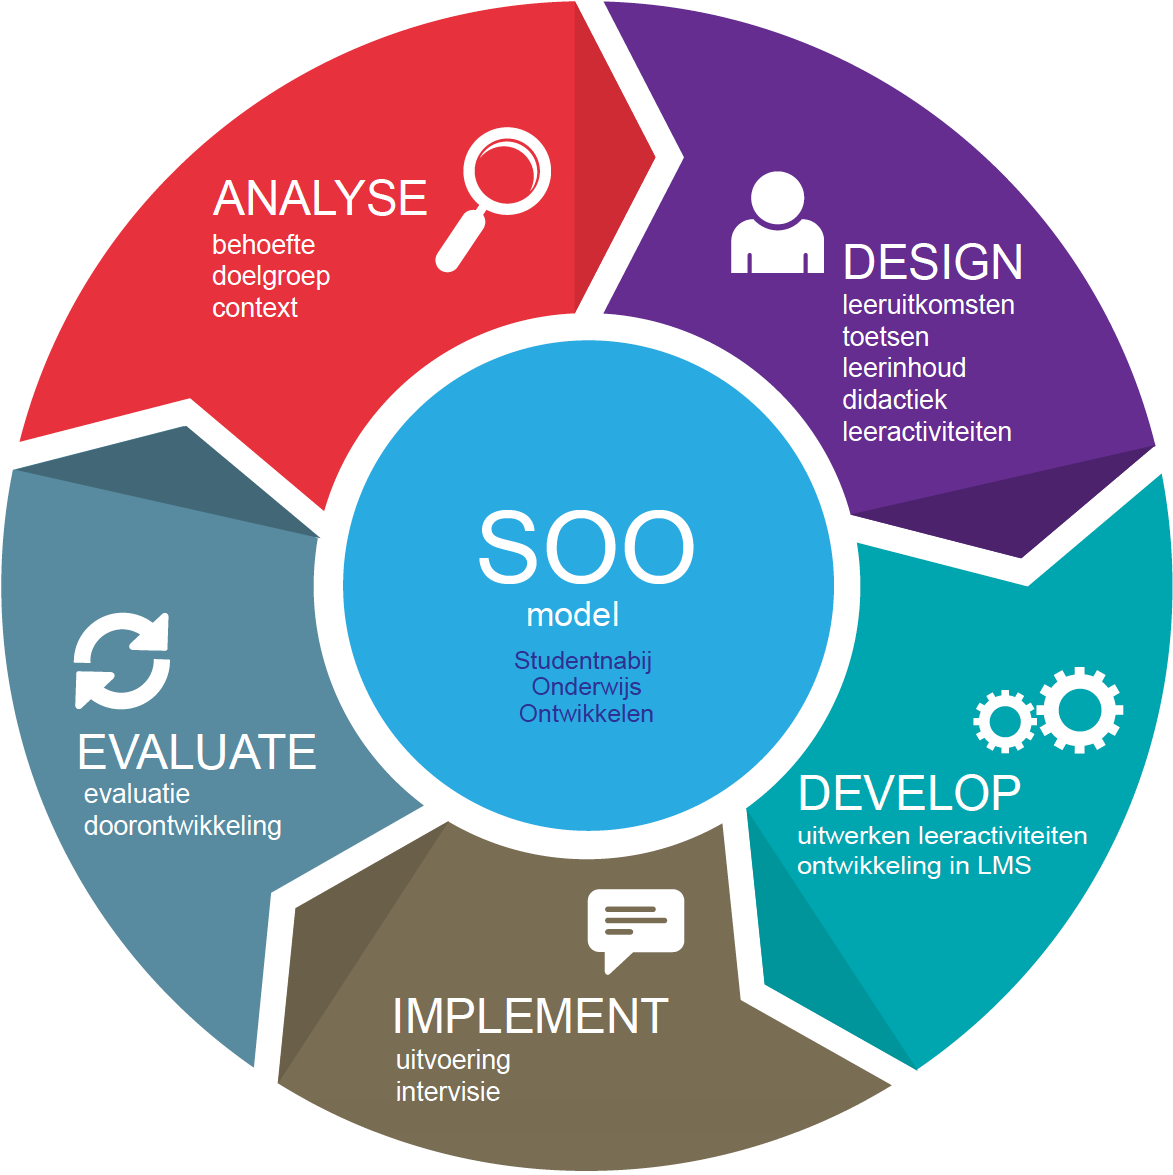
\includegraphics[width=0.5\textwidth]{figures/SOO_model.png}
%     \caption{Graphical representation of the \acrfull{soo} model (source: \url{https://portal.fhict.nl/medewerkersplein/Didactiek/Pages/Didactiek.aspx})}
%     \label{fig:SOO}
% \end{figure}


\subsection{Analyse}\label{chapter:didactics_phase_analyse}\label{chapter:didactics_phase_analyse}
Initially, the needs of students and the professional field are considered. My personal experience with \acrfull{pie} through student internships is in fact one of the reasons to develop a writing skills module. Generally, \acrshort{pie}'s feedback on written tasks boils down to \textit{informality in style }and difficulty to provide a \textit{smooth flow of ideas}. Furthermore, many alumni indicate struggles in the writing tasks, especially during the graduation. I am myself a \acrshort{fhict} alumna and I recognize similar lack of information.
\\\\
In my opinion, the most suitable audience for the writing skill module workshop are Semester 3 and Semester 6 students, respectively.
Both semester are in fact before the two internships, which are the two study unites heavily dependent on writing tasks. Furthermore, the students already acquire prior knowledge about the required content of the writing tasks within the project of ICT \& Software Engineering Semester 2, tasks which are repeated in the following semester, during a similar project involving \acrshort{pie}. Furthermore, additionally to the practice and experience of prior semesters, with Semester 6 the focus on research would increase, thus, so would the complexity of the the writing tasks.
\\\\
The writing module can be integrated in ICT \& Software Engineering Semester 3 as supportive workshop. While the development of Semester 6 is not yet started, I predict a similar context.
%Initially, a general picture of the course current situation was depicted, analyzing the \textit{target audience}, their \textit{needs} and the \textit{context} in which education is being developed. 
%Some example personas described in~\cref{appendices:personas} were composed to better understand the target audience.
%While the course is a fourth year elective, throughout my experience as an \acrshort{ale} teacher students that did not manage to find an internship project (thus, are half way in their third year) are usually joining electives to not waste an academic semester. 
%However, as a forth year ICT \& Software Engineering elective, \acrshort{ale} targets young professionals with a strong technical background, stimulated by applied mathematics and software engineering. 
%Preferably, \acrshort{ale} students should have studied in the ICT \& Software Engineering or ICT \& Technology profile and should have completed at least the first two academic years. For more details about the \acrshort{fhict} program see \cref{appendices:curriculum_structure}. 
%Furthermore, the needs of both the students and the professional field were considered, where solid software engineering competences were recognized essential, especially as an \acrshort{ict} graduate.
%Therefore, course material development would not imply changing the course structure, but \textit{clarify and enrich the learning experience}.
%As a consequence to the analysis, the context (such as instructional materials, learning environment) was realized and it is further described in the next section.

\subsection{Design}\label{chapter:didactics_phase_design}\label{chapter:didactics_phase_design}
\subsubsection{Learning outcomes}
For the writing skill module workshop I propose an additional learning outcome in each semester, namely communication in a written format.

\begin{figure*}[h!]
\begin{tabular}{|p{\textwidth}|}
 \hline
    \textbf{Learning outcome Semester 3: Basic communication writing skills}\\
    Communicate in a specific written task in the most appropriate manner.\\
 \hline
    \textit{Explanation}\\
    You use basic stylistic considerations and you are aware of your stylistic choices.
    \\ 
    You communicate information smoothly, using logical connections between ideas.\\
 \hline
\end{tabular}

\begin{tabular}{|p{\textwidth}|}
 \hline
    \textbf{Learning outcome Semester 6: Advanced communication writing skills}\\
    Communicate in a specific written task in the most appropriate manner.\\
 \hline
    \textit{Explanation}\\
    You use an appropriate/predictable format/pattern for a particular type of text (e.g. summary, introduction, data commentary).
    \\ 
 \hline
\end{tabular}
  \caption{Learning outcome for Semester 3 and Semester 6}
\end{figure*}

\begin{figure}[h!]
    \centering
   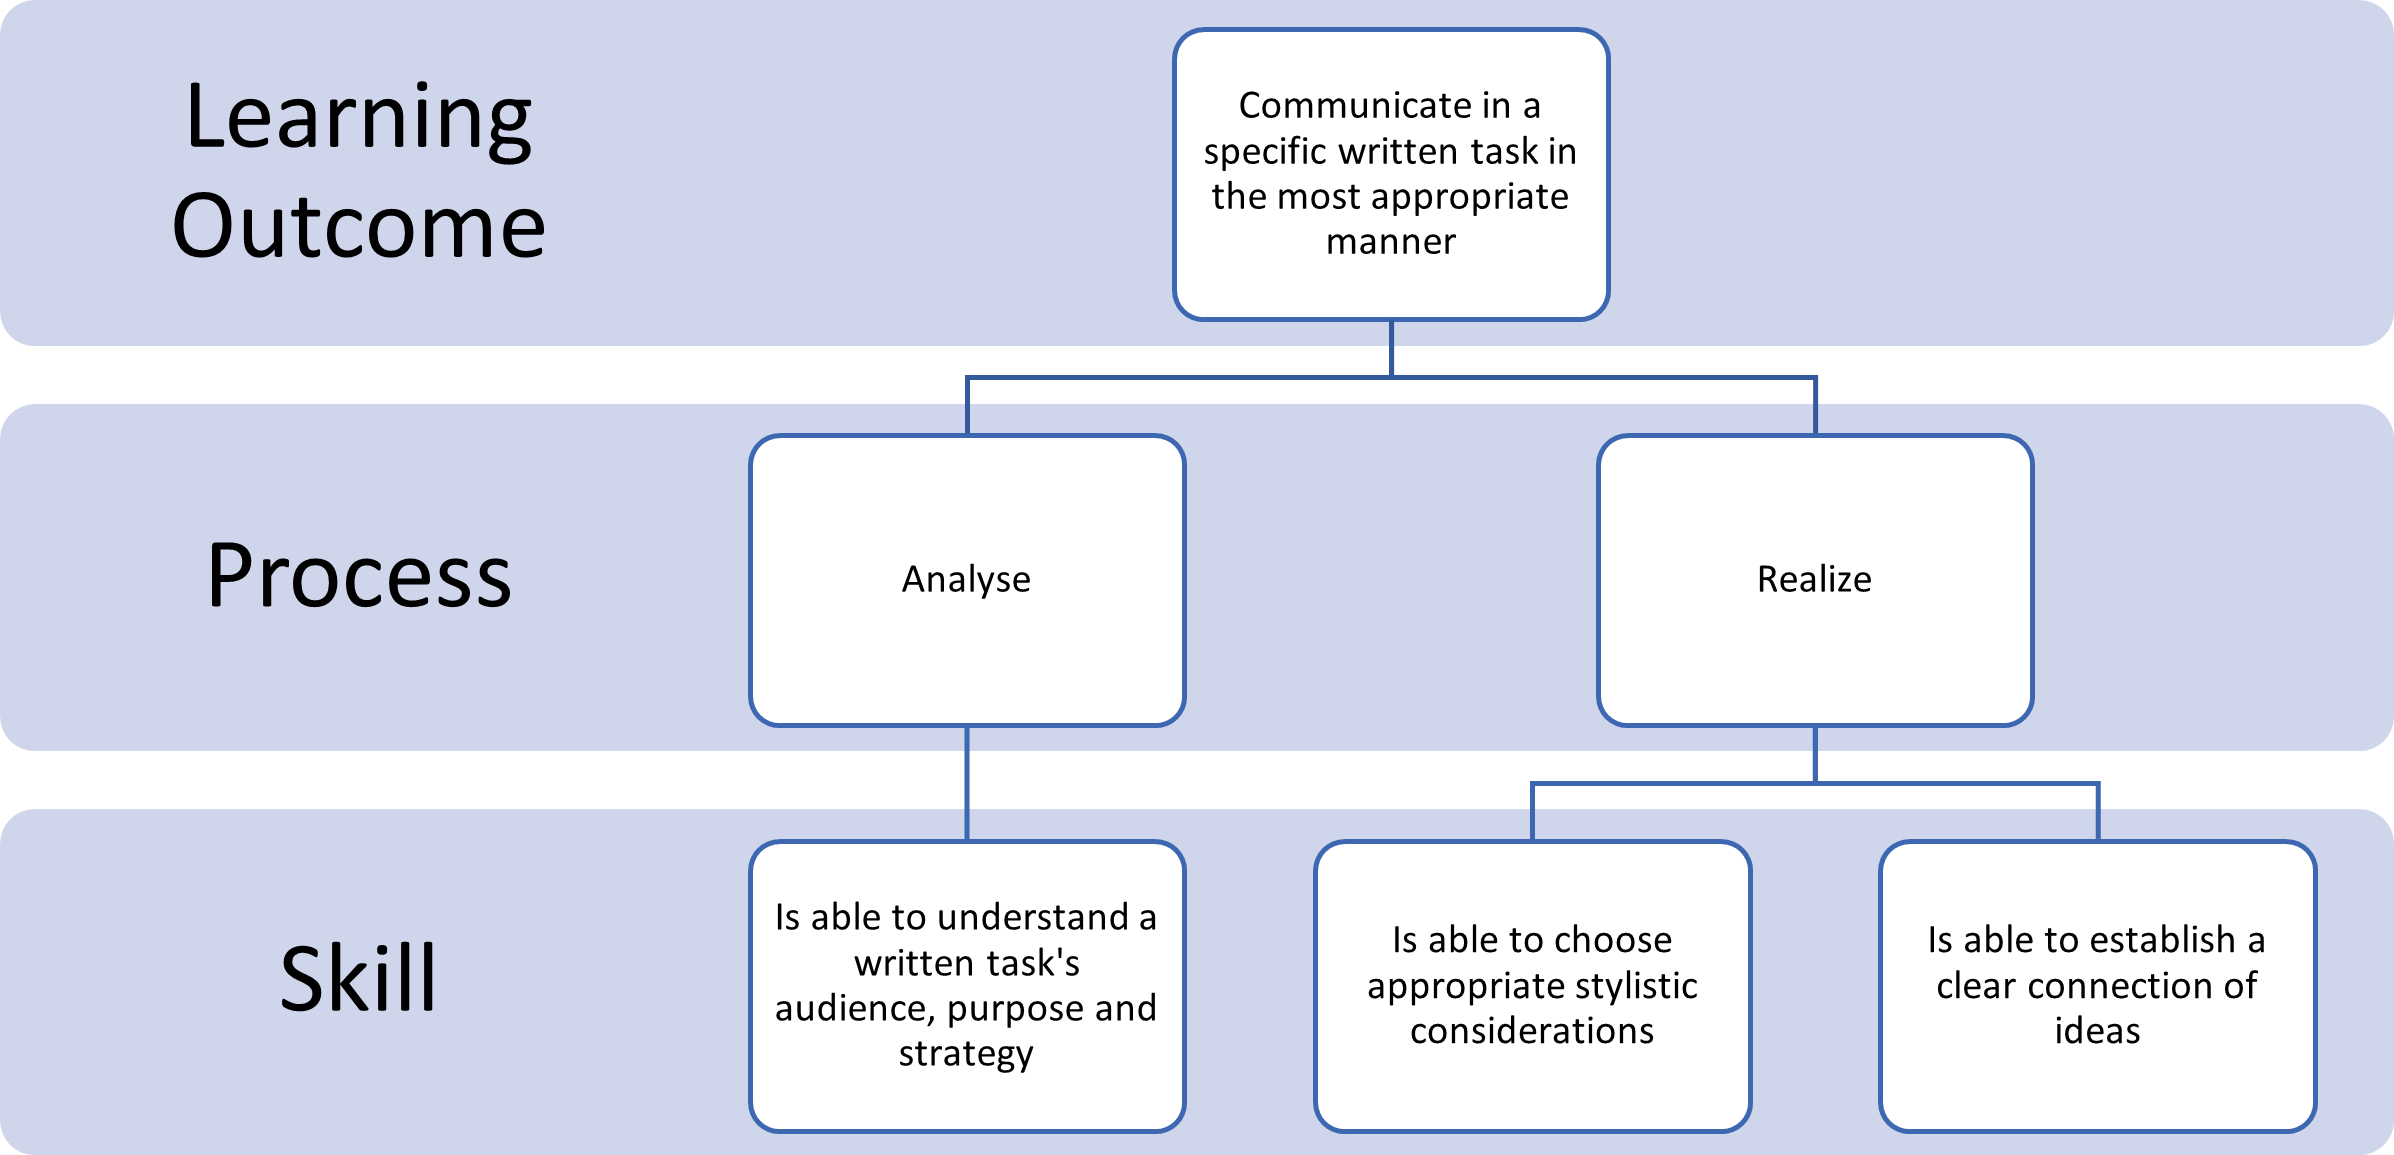
\includegraphics[width=\textwidth]{appendices/learning_outcomes/LO_S3.png}
    \caption{Skill tree for Semester 3 learning outcome: Basic communication writing skills}
    \label{fig:LO_S3}
\end{figure}

\begin{figure}[h!]
    \centering
   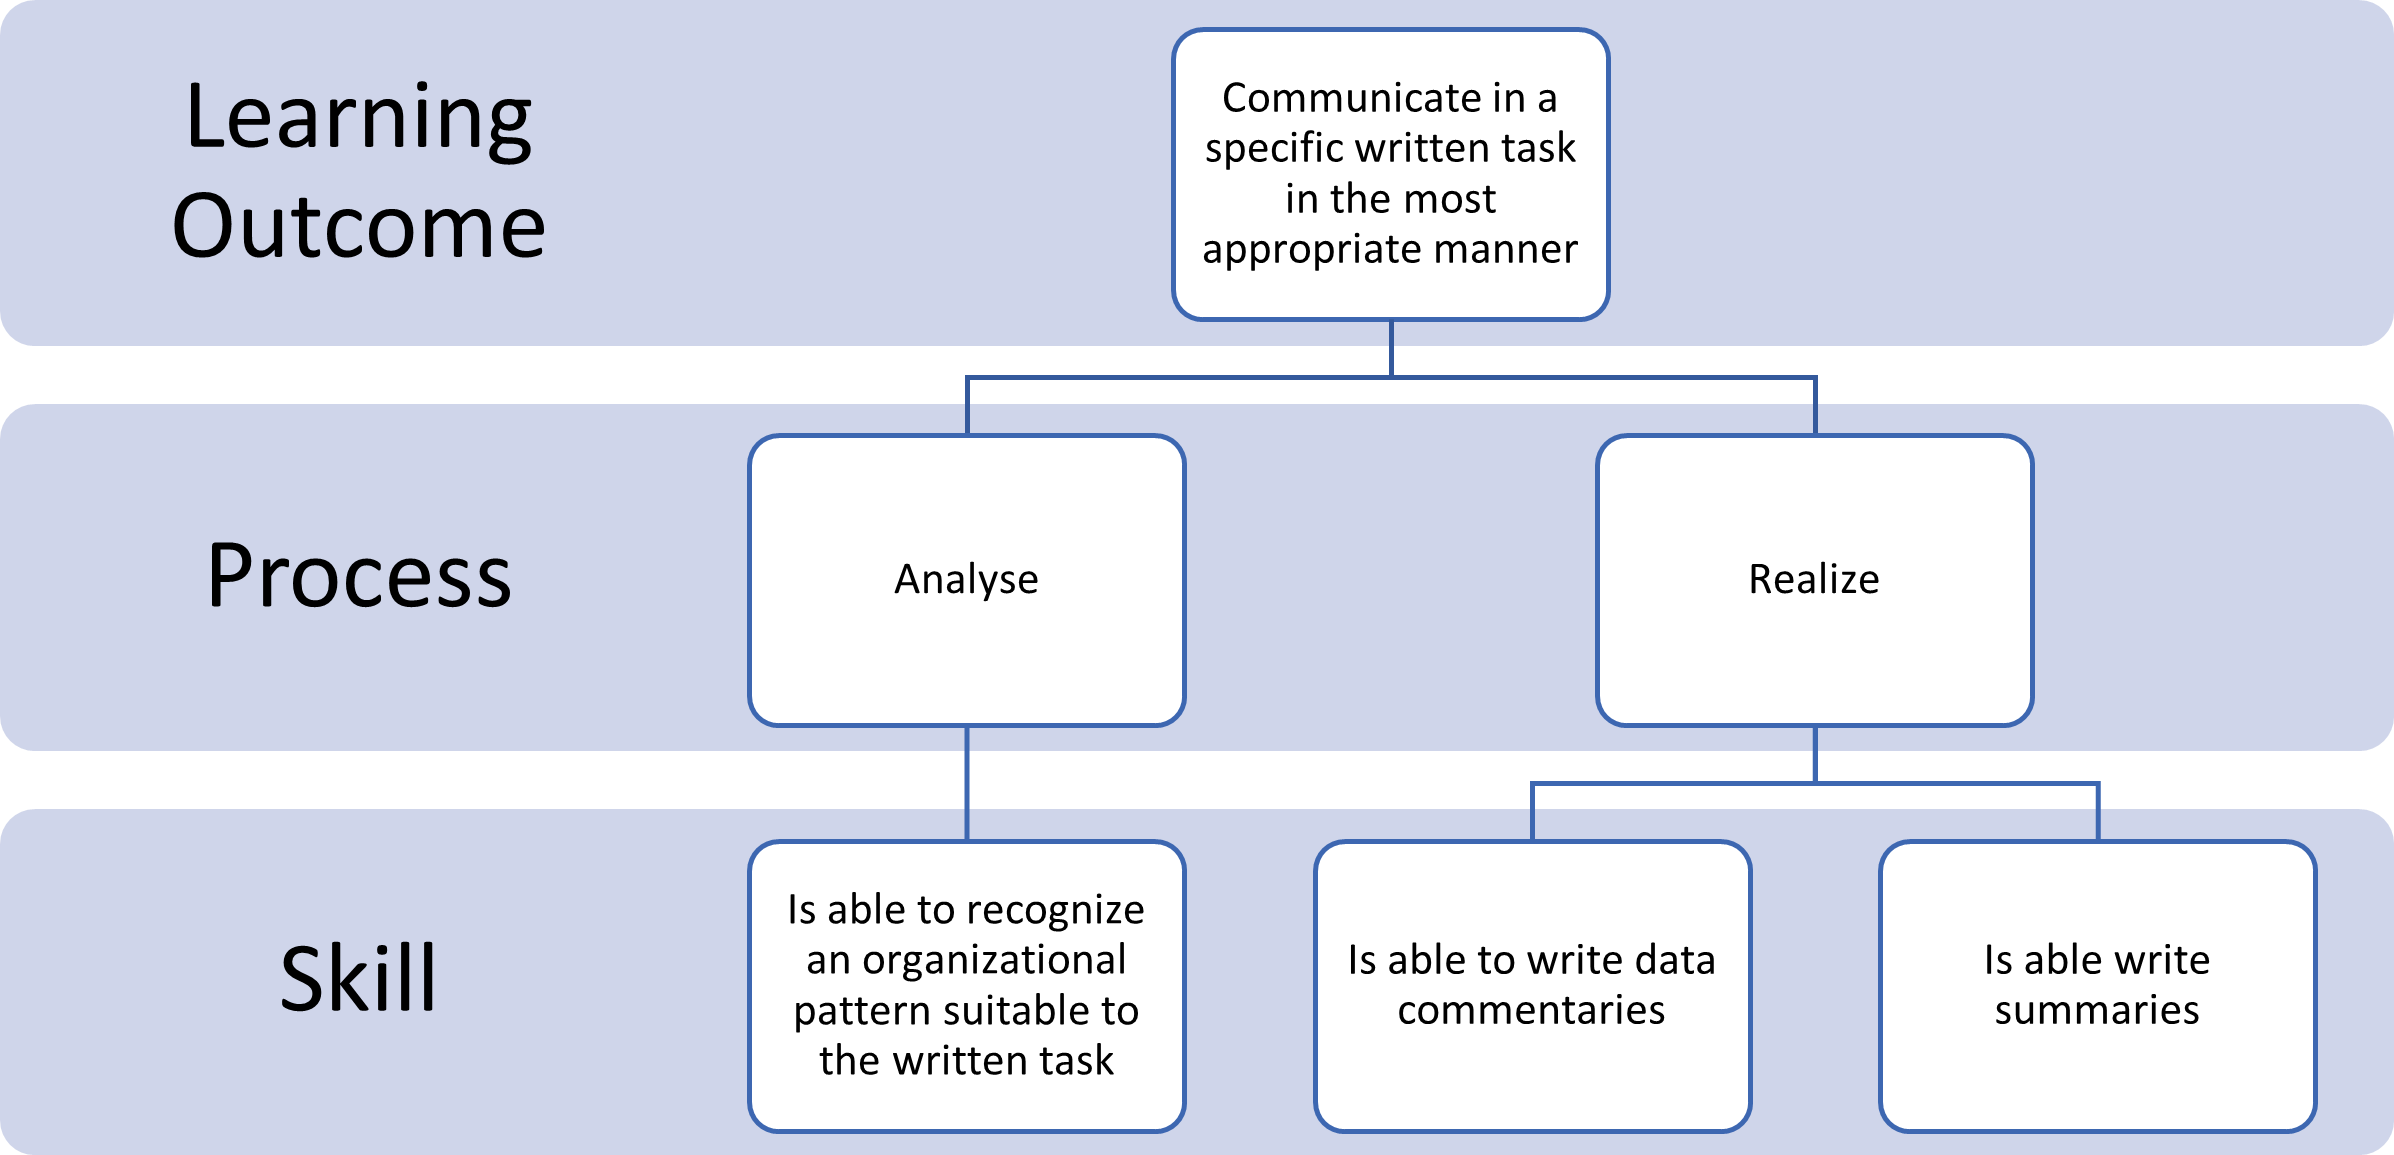
\includegraphics[width=\textwidth]{appendices/learning_outcomes/LO_S6.png}
    \caption{Skill tree for Semester 6 learning outcome: Advanced communication writing skills}
    \label{fig:LO_S6}
\end{figure}

\subsubsection{Learning activities}

The employed teaching method closely follows the \acrshort{4cid} model~\cite{FHICTTeachingMethods}. This model describes four basic components fitted to the course as follows:
\begin{itemize}
    \item learning tasks (weekly theory and practical lessons)
    \item supportive information (course notes and worked out examples, explanation of basics)
    \item practice tasks (individual tasks that aid to better understanding of topic)
    \item procedural information (feedback and feed forward through weekly individual short progress meetings)
\end{itemize}


\subsection{Develop}\label{chapter:didactics_phase_develop}\label{chapter:didactics_phase_develop}
Subsequently, the course material development followed. 
While original topics and assignments were preserved, only instructional materials were reworked.
Having rather considerable experience with the course subject, the task of developing lesson material suit me well. 
Furthermore, I have had the experience of fine-tuning instructional materials previously for other courses. The deliverables from this phase were:  
\begin{itemize}
    \item lesson slides
    \item assignment and supportive information (course notes)
    \item practice assignments
    \item \Gls{canvas} master course
\end{itemize}
While I could adapt and reuse former assignment examples, the majority is developed from scratch. 
I also added practice assignments (additional exercises) as a preparation for the assignment. 
Furthermore, example solutions of the assignments were constructed to aid future course teachers and reduce their preparation time.\\\\
A sample presentation along with the corresponding assignment and supportive information is provided in~\cref{appendices:slide_assignment_info}; this appendix includes also a sample solution and corresponding code snippet. 
An example of a \Gls{canvas} page is also attached in~\cref{appendices:slide_assignment_info}.\\\\
The most challenging task was to develop appropriate examples and practice assignments which would provide the basic understanding and would still require further self-engagement from the students.
Furthermore, researching trusted sources for further reading proved to be more time-consuming than expected. 
However, this experience has turned out to be quite enjoyable, and in the future I am looking forward to other development opportunities, even curriculum development.

\subsection{Implement}\label{chapter:didactics_phase_implement}\label{chapter:didactics_phase_implement}
The redesigned course material was first offered in the second half of the Fall semester 2020-2021, specifically for \acrshort{ale}2 which is about the automata topic. 
Due to the COVID-19 outbreak, within \acrshort{fhict} the lessons were \textit{blended}: online and face-to-face. In fact, according to a study by~\citet{blended2013}, the combination of blended learning produces stronger student learning outcomes than learning solely through face-to-face instruction. Another advantage of the online education is the possibility to record the theory parts of the lessons and make them available for revision. Further description of the use of technology during COVID-19 is given in~\cref{chapter:tel}.



\subsection{Evaluate}\label{chapter:didactics_phase_evaluate}\label{chapter:didactics_phase_evaluate}
To evaluate the effectiveness of the redeveloped course materials, the \acrshort{ale} Fall semester 2020-2021 students were first offered the old variant in \acrshort{ale}1, and the reworked variant in \acrshort{ale}2. Further description of the evaluation is presented in~\cref{chapter:research_expertise}. 


\section{Reflection}\label{chapter:didactics_motivation}
Developing course material has been an enlightening experience. 
While I vaguely knew about the faculty's policy and employed didactical methods, I learned about many new aspects that define education within \acrshort{fhict}. 
\\\\
Firstly, learning about the HBO-i framework has helped me better understand the expected competencies at a certain time in the study.
While I was aware of the increasing level of proficiency in each semester having attended similar education, previously, I only assumed the expected competencies and skills. The HBO-i framework offers an easy to follow separation of professional tasks and expected skills, which can be easily translated into the a course.  
Furthermore, the framework has helped me improve the quality of the already existing learning outcomes, as well as introducing a new learning outcome, namely documentation, essential in the final year of \acrshort{hbo} education. 
\\\\
Secondly, learning about a \acrshort{fhict} standardized procedure of defining learning outcomes has helped me provide consistent course design. 
I believe that consistency is key to delivering education. 
Students acquaint with certain standards which, if consistent, can ease learning within an institution's education, as students would expect similar requirement formulations and definitions, although on different topics and difficulty levels. 
While this is not the case in the old curriculum, I believe that the new curriculum is respecting these learning outcome standards and provides consistent education.
\\\\
Another important insight I learned while developing course material is the \acrshort{4cid} model for conveying knowledge through theory and practical materials. 
As I quickly realized I was already adopting to this model in my way of teaching, I was pleased to learn it is applied quite often within \acrshort{fhict}, especially in the new curriculum.
While the learning model may vary as the students progress in their study, I believe at least in the first academic year is ideal to have consistent education.
In addition, while researching didactics within \acrshort{fhict}, I also learn about the demand-based variant. 
This gave me some basic knowledge of the structure of this variant, which helps me better explain first year course-based English stream students what is the difference between the two variants.
\\\\
Lastly, I learned about the \acrshort{soo} model and how to properly conduct course development. 
I have re-developed many courses (e.i. theory slides, demo examples, mock exams and exams content) throughout the four \acrshort{fhict} academic years, always thriving to provide learning materials according to the students feedback.
However, I think having such a model, once again, provides consistency in the institute's education and eases a student's experience throughout the learning process. 
\\\\
Overall, I enjoyed and the entire course development process and I have already been offered to contribute to the development of the new curriculum semester six, which I accepted enthusiastically.

\clearemptydoublepage

\chapter{Testing}\label{chapter:testing}
Assessment of the ICT \& Software Engineering elective \acrfull{ale}.

% \section{Choice and justification of testing methods}\label{chapter:testing_choice_justification}
% A student-centered education envisioned by \acrshort{fhict} requires a student-centered assessment~\cite{FHICTAssesmentPolicy}. 
This implies frequent \textit{formative feedback} and \textit{feed forward} for the students throughout their learning process. 
\textit{Formative assessment}, thus, benefits not only the students, but also the lecturer, who can get a better picture of the student and his development during the education by collecting and interpreting information on the student performance.\\\\
While the learning outcomes for the \acrshort{ale} elective defined during the design phase in~\cref{chapter:didactics_phase_design} form the basis of the integral assessment, weekly teacher feedback is aimed to appreciate ongoing development and performance.
For that reason, the assessment consists of smaller components which at the end form an integral assignment.\\\\
From the first iteration of the course, I realised that students were either not attending the formative feedback sessions or not actively working on the course topic due to various reasons. 
This ultimately yield to a rather poor integral assessment. 
Considering this outcome, in the concurrent iteration of the course I made the formative feedback sessions mandatory.
I asked students to submit their weekly progress or shorty describe their reason of delivering up to mark. However, the performance did not significantly change, rather worsen.
In~\cref{appendices:scores} a histogram of the integral assessment scores and the significance difference test score is shown. Another aspect to consider about the course is that it is an elective, thus, students may have various reasons to participate, as shown in the recent course survey in~\cref{appendices:survey}. Throughout the course iterations I also noticed many students usually drop \acrshort{ale} after the first two weeks, as they cannot fit the workload with their rest of the educational path/personal life, although always advised even from the fist lesson (some students are doing their graduation and are looking for opportunities to fill in the last 3\Gls{ec}s or some are free-riders due the format of the course, e.i. no exam). Therefore, the mandatory weekly formative assessment was left out in the end.

% \section{Assessment construction}\label{chapter:testing_assessment_construction}
% \subsection{Basic design}\label{chapter:testing_basic_design}


\begin{figure}
    \centering
    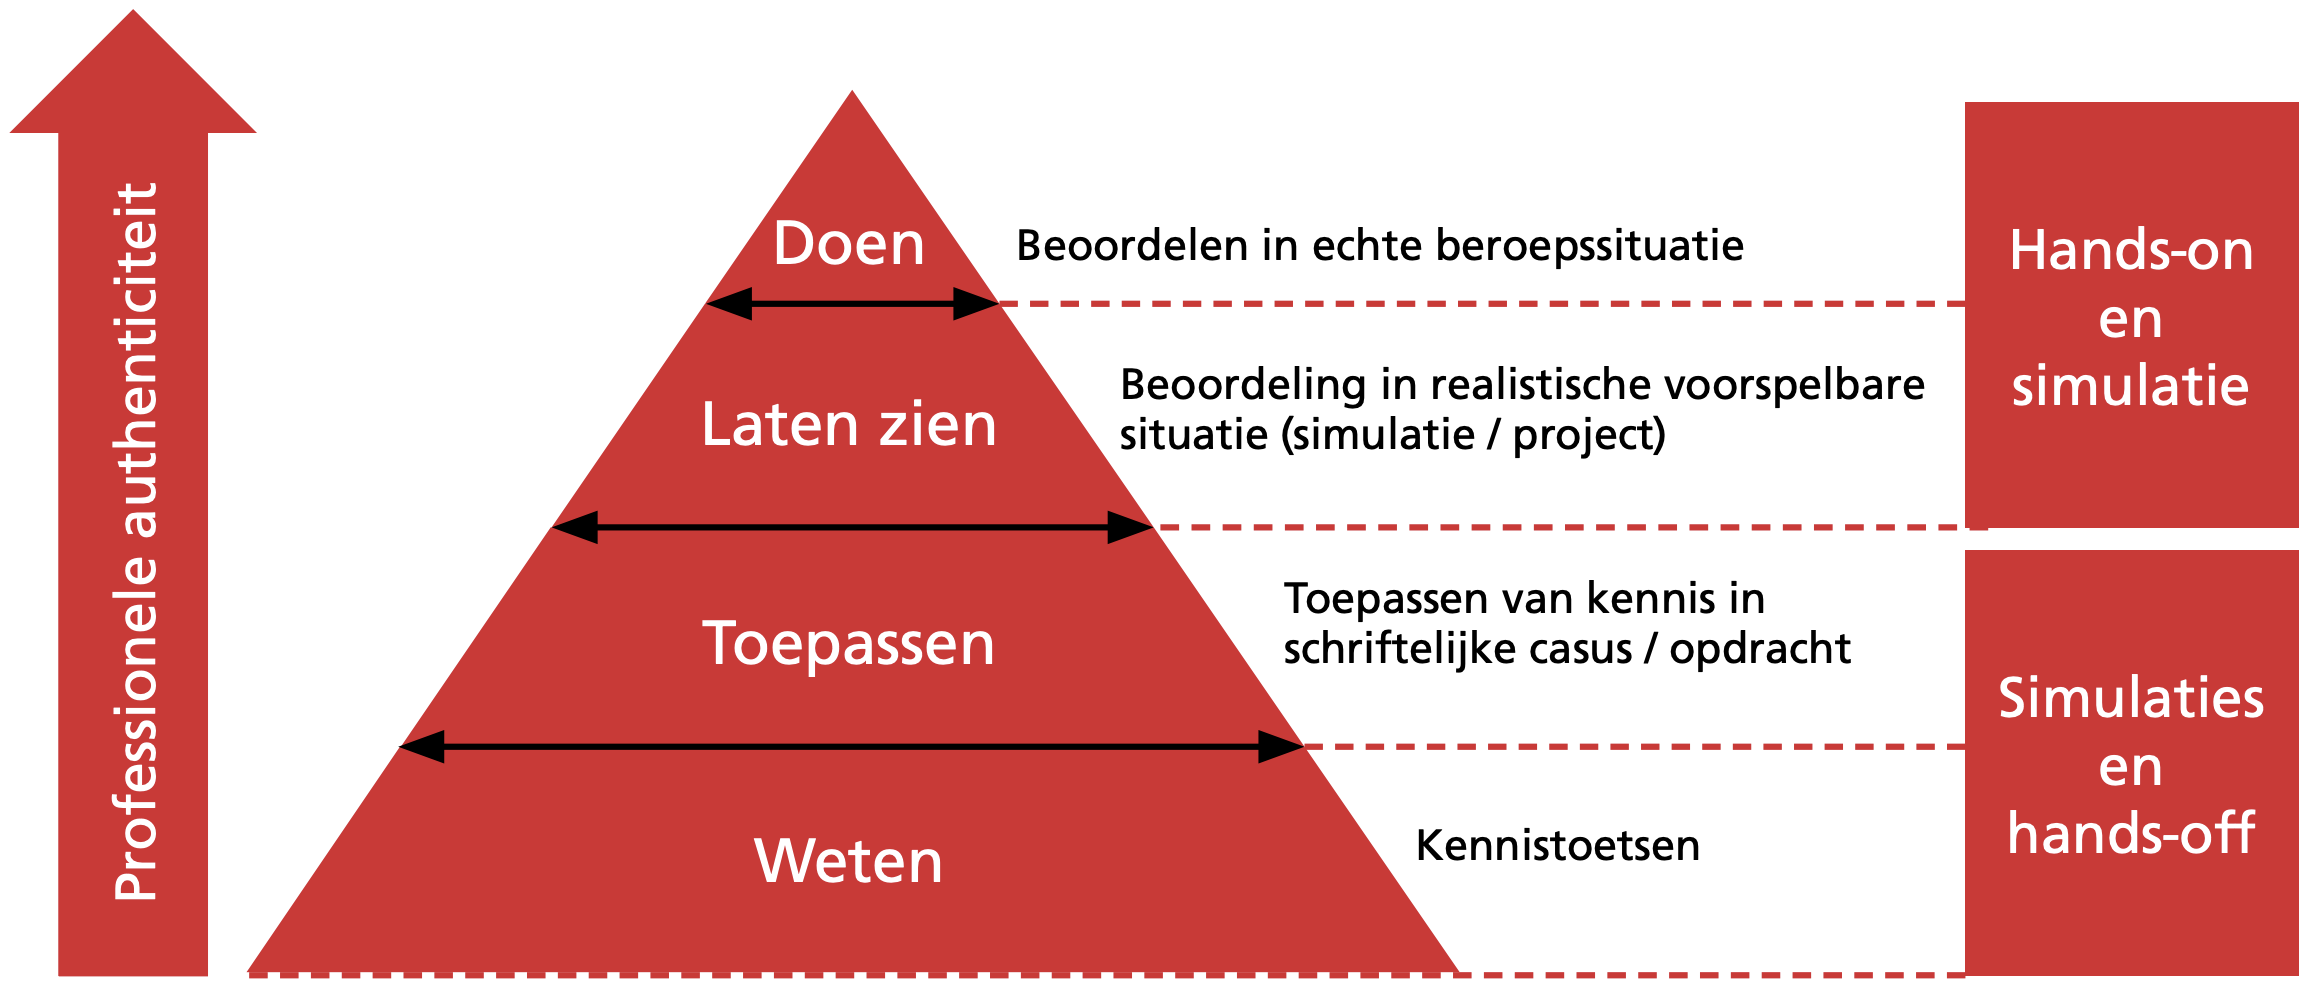
\includegraphics[width=\textwidth]{figures/miller_pyramid.png}
    \caption{Miller's pyramid~\cite{toetskwaliteit2014}}
    \label{fig:miller}
\end{figure}

While the assessment matrix and guidelines are essential to ensure a correlated assessment throughout the students, I was surprised to find out from the first iteration of the course that it was missing. 
I believe that these components do not only validate the assessment but, together with the learning outcomes, it also helps the students to gain insight into their learning process. 
Furthermore, by explicitly describing and publishing assessment criteria and bringing it to the attention of students, the assessment becomes transparent, a crucial assessment quality criteria.
\\\\
After analysing the test quality principles, a test program was developed. The Miller's pyramid which layers student progress from testing cognitive skills to practical performance was employed~\cite{toetskwaliteit2014}. 
A graphical representation of this program is shown in \cref{fig:miller}. 
At the bottom of the pyramid, the testing program implies test formats that build the knowledge base.
As the student progresses up the pyramid, the complexity and authenticity is shown through practice and performance of professional tasks.
However, the pyramid levels do not have to be sequentially followed from bottom to top. 
%This does not mean that the levels in the pyramid are sequentially from bottom to top must be finished above. Students may first "do" something and then only start to acquire the necessary knowledge. All this depends on learning style and vision learning and the complexity of the assignment.
\\\\
\Cref{appendices:assessment} contains all developed assessment documents: \textit{guidelines}, \textit{test matrix} and \textit{assessment criteria}. Apart from the specific course topic assignment, learning outcomes objectives are also considered, all accounting equally to a total of 100\%. 
Students are also assessed on their own contribution apart from the predefined assignment requirements, as a result of \gls{scaffolding}.

\subsubsection{Some examples}
After the first week, students are expected to deliver the core architecture of the application, which implies reading input from the front end and producing an output. The following work is expected:
\begin{itemize}
    \item software engineering (including inital \acrshort{uml} diagram of the proposed solution)
    \item handling of third party tooling GraphViz
    \item unit testing 
\end{itemize} 
These deliverables are re-worked thought the project and enhanced with new features. The feedback session after the fist assignment is essential in understanding studnet's competences and feedfroward for following assignments. Especially in \acrshort{ale}2 the final assignment is dependent on proper software architecture refined throughout the prior assignments to properly implement it. 

\subsection{Feedback and assessment}\label{chapter:testing_assessment}
Although the course was held during the lockdown, the feedback was done online. I gave formative feedback to students remotely through online meetings or through \gls{canvas}. This is detailed in  \cref{chapter:tel}.
Formative feedback helps students in stirring progress in the right direction. The course assignments are rather complex and rarely the lessons and course material suffice in proper understanding for students~\cite{feedbackFHICT}. In fact students long for quick feedback on their work to reassure their work is not whitout success. While I strive to provide constructive feedback, this covers both positive and negative feedback. An example of formative feedback is shown in~\cref{appendices:feedback}.\\\\
Subsequently, summative feedback together with the assessments for the final project submitted at the end of the course helps students identify improvement points. Usually, assessment is less unexpected, as students are aware of their progress and improvements points throughout the course.

\subsection{Evaluation}\label{chapter:testing_evaluation}
Although the course started with ten students, in the end only one student completed the course. After discussion, I concluded many students decided to join less time consuming courses and spend the rest of the time working on the side. While this was a situation that could not be predicted, the course being an elective after all, a comparison between the old and the new course materials cannot be statistically analysed anymore. However, a statistical analysis is shown in  \cref{chapter:research_expertise} containing an extensive study over the student performance on the basis of course material from 2017-2021.\\\\
Only the student that completed the assignment provided an evaluation over the new course material in written form. Based on the studnet's written evaluation, also shown in \cref{appendices:evaluation}, I concluded that the way the course manual (syllabus) was presented in \acrshort{ale}2 is preferred. Furthermore, as the student enjoyed the subject (joined both \acrshort{ale}1 and redesigned \acrshort{ale}2), I value this opinion highly. A remark the student highlighted is the need of more examples. These were already added in the new syllabus, but more detailed examples are expected. While I do not entirely agree with this recommendation, I understand the inconvenience the students go through in designing their own input examples. In fact, part of this project is that students create their own examples and test with each other the outputs. Given the fact that the \acrshort{ale}2 Fall 2020 student was left alone in the class, creating own examples and testing is less reassuring. However, I will consider this once again, and try to elaborate more examples for the next iteration.



% \section{Reflection}\label{chapter:testing_reflection}
% Developing testing materials throughout the redevelopment of \acrshort{ale} I learned about many new aspects that concern an assessment within~\acrshort{fhict}. First and foremost, I learned about the assessment policy~\cite{FHICTAssesmentPolicy}. While before I was only assuming what should be considered when developing and undertaking an assessment, learning about the \acrshort{fhict} assessment policy has made me a better assessor. Specifically, the policy provides a set of rules and regulations that must be followed to not only guarantee consistency but also quality of the assessment within the institute. Furthermore, the quality criteria described in the assessment policy helped me confirm the inconsistency of the previous \acrshort{ale} variant assessment, where assessment transparency was completely missing (e.i. students did not know how they were being scored and based on what learning outcomes).\\\\



\clearemptydoublepage

\chapter{TEL}\label{chapter:tel}
Advances in \acrfull{ict} have revolutionized learning
and assessment both within and outside of classrooms. This section describes the employment of technology to enhance education.

% \section{Scope of technology in education}\label{tel_scope}
% \Acrfull{tel} refers to technology-based learning and instructional systems through which students acquire skills or knowledge, usually with the help of teachers and technological resources (e.i. computers, smart devices)~\cite{tel2005}. 
From face-to-face education to e-learning, technology plays an important role in enriching the student's learning experience. Within \acrshort{fhict}, technology is the primary tool with which education is being carried out. 
Furthermore, due the recent COVID-19 outbreak that caused the transition towards blended education (e.i. combination of online and face-to-face education),  technology has become indispensable.

% \section{Face-to-face education}\label{tel_face_to_face}
% Normally, lessons are given face-to-face, where the teacher conducts instruction with the aid of digital tools. 
Furthermore, information is also made available digitally through online platforms.   
On overview of these tools follows.

\subsection{Canvas}

At \acrshort{fhict}, \Gls{canvas} is the the primary \acrfull{lms}, gradually replacing the former platform \Gls{sharepoint}. 
\acrshort{lms}s are defined as a type of software application where programmed instructions drive all learning activities; furthermore, they act as a repository where learning resources can be stored~\cite{lms2020}. 
In particular, \Gls{canvas} offers a series of features, from information communication (e.i. theory and assignment publication) to assessment and progress tracking by means of grade book (e.i. formative and summative indications). 
Moreover, \Gls{canvas} is highly customisable, making it a flexible environment for both the teachers and students.
I regularly utilize these feature in my teaching activity and I also guide students in navigating the platform. 
Having experience with the former \acrshort{lms}, an advantage of \Gls{canvas} is that it helps students to organize in a timely manner, providing notifications about upcoming assignments and deadlines for enrolled courses. 
This feature does not exist in \Gls{sharepoint}, teachers usually having to revert to publishing announcements onto the main page. 
However, this was not efficient as students would see announcements of courses they were not enrolled to and would be overwhelmed with redundant information.
Another advantage of \Gls{canvas} is that it provides a centralized assessment system. 
Previously, assignments were handed through emails and the assessment was published as a \Gls{mexcel} spreadsheet. 
Furthermore, due to the disrupted communication, feedback was less digital. 
An example of an assignment assessment and feedback with \Gls{canvas} is shown in~\cref{canvas_assessment_feedback}.

\subsection{Other tools}
Instructions are primarily guided through \Gls{mppt} slides. 
I often invest time animating components in my presentations, especially to emphasize a process or a method. 
As \citet{ppt2011}  study showed, lower textual density in slides and added non-textual elements appear to stimulate positive student feedback. 
Furthermore, I also utilize slides to engage students and initiate discussion. 
Some example slides are shown in~\cref{appendices:slide_assignment_info}.\\\\
To stimulate students further, I frequently run theory quizzes using \Gls{kahoot}. This is a web-based student response system that engages students through game-like premade or impromptu quizzes, discussions and surveys and can be easily accessed from any device such as iPad, Android device, or Chromebook~\cite{kahoot2015}. According~\citet{icard2014} and many other studies, game-based learning is considered a best practice in education. An example of a \Gls{kahoot} quiz is shown in~\cref{appendices:kahoot}.\\\\
Assignments or document templates are usually written as a \Gls{mword} document and published as a \acrshort{pdf}. 
I also endorse \gls{latex}, another software system for text document editing, especially for more advanced students (e.i. internship and undergraduate students in the final bachelor's year). \gls{latex} is based on the philosophy that authors should be able to focus on the content of what they are writing without being distracted by its visual presentation~\cite{latex2014}, which is usually the case with other text editing tools like \Gls{mword}. 
To ease student's introduction to \gls{latex}, I created a document template which is publicly available in \Gls{overleaf}, as shown in~\cref{appendices:latex}.\\\\
For software development, the version control system \Gls{git} is usually used to track code changes. 
Students usually set up and administer a \Gls{git} repository and then a link is further shared. 
This tool is especially convenient for projects, either grouped or individual. For instance, while not mandatory, I endorsed \gls{git} to \acrshort{ale} students as a simpler way of sharing their source code for feedback, instead of uploading archived folders to \gls{canvas}.\\\\
Although Canvas offers communication channels, audio-visual communication is lacking; therefore, I decided to introduce another platform, \Gls{slack}. 
This idea evolved as a way to unite and stimulate student discussions on course topics in an online environment. 
Before the COVID-19 outbreak and the migration to online learning, I have used \Gls{slack} with all the four scholarly year students. First, I saw great opportunities to group students in one platform (other than WhatsApp and Facebook) and discuss solutions to \acrshort{ale} assignments. Then, I introduced \gls{slack} to my mentor first semester students as a platform to acquaint and discuss education related topics, also including, but not limited to, personal issues with respect to moving and living in the Netherlands. Currently this platform is replaced by \acrshort{fhict} with another officially administered platform for online lessons during the COVID-19, presented in the following section.  


% \section{Online and blended education}\label{tel_blended}
% Due to the recent COVID-19 outbreak, at \acrshort{fhict} education has shifted to online. 
From March to June 2020 education has taken place online exclusively. However, since the start of the academic year 2020-2021, education is blended, e.i. students have partially online and face-to-face classes.
While this choice is purely a necessity to ensure the continuation of education in the context of a pandemic, blending instructional materials with online interventions can be a better setting as opposed to fully online or face-to-face mode of instructions, if done well~\cite{blended2020}. 
In that sense, technology it is not just a vital necessity but also an asset. 
\\\\
In addition to already existing technology such as \Gls{canvas} and \Gls{git}, at \acrshort{fhict}, online lessons are offered via \Gls{mteams}. 
An advantage of \Gls{mteams} is that it provides a solution for both synchronous and asynchronous learning. 
Just as a physical classroom has a specific schedule, using this application it is possible to provide live online lessons at a pre-scheduled time. The platform can also be connected to the regular email and schedule services from Outlook, students being one click away from joining the lessons from their calendars. Moreover, lessons can be recorded for students to review at a later time. With almost one year of education offered fully or partly online, many students have mentioned the advantage of recorded lessons to better prepare for assessments (for instance exams).\\\\
A challenge in the online environment is the visual engagement. Unlike face-to-face, in an online lesson it is challenging to sense student engagement or receive feedback about their understanding. Recently, \Gls{mteams} has been releasing features such as "Rise your hand" and "Together mode" which improve the overall communication channel and make the online environment more physical. Furthermore, the Polly extension of \Gls{mteams} to manage voting options is a tool I make use of on a regular basis for polls and opinion gathering. \Cref{appendices:ms_teams} shows some examples of conduction lessons in \Gls{mteams}. 





% \section{The downside of technology in education}\label{tel_downside}
% Despite the rapid technological advancements, education is facing some problems.
First and foremost the internet as a source of information poses a threat to the learning behavior of students.
While the source of information is endless, it is not necessarily accredited.
Excessive learning individualization through online means may lead to the denial of teacher-student or professional-apprentice dialogue. 
For example, during internships many students get consumed into the online research and individualize their process, thus, missing consulting the company. This is especially the case for students performing internships during the COVID-19 pandemic, where regular activities at the company are carried out online.\\\\
Furthermore, new technology creates new issues in terms of cheating and plagiarism.
Although the internet has helped to accelerate the research process for many academics, it has also created easy access to methods of cheating and plagiarism for students~\cite{downside2006}.
For instance, students would rather copy already existing solutions from various online forums such as \gls{stackOverflow}, rather than spending time solving the problem themselves, thus, missing the practice. This is the case for many student in the \acrshort{ale} course for which there are solutions available online. Thought my experience in teaching this course, I identified many cases of fraud with an internal plagiarism check tool.\\\\
Apart from damaging practical skills such as paper writing or arithmetic, excessive use of technology also leads to reality disconnection. Students are dependent of their electronic devices; therefore, their attention to the surroundings decreases. While the lessons at~\acrshort{fhict} usually require the use of technology, it is students responsibility to avoid distractions and cooperate with the teacher for a good learning atmosphere. 



% \section{Reflection}\label{tel_reflection}
% As I consider myself a fast learner, I employ \acrshort{tel} effortlessly. Especially my recent experience as an alumna in similar education has fortified my \acrshort{tel} skills. 
Having used both \gls{canvas} and \gls{sharepoint} during my studies, identifying and implementing familiar features was straightforward. 
Even the generation of production courses within \gls{canvas} (e.i. generate a start-up version of a course for new students every semester, including new deadlines and updated course materials), although a new feature, was manageable by myself.
\\\\
\acrshort{tel} has definitely revolutionized education, allowing online means to learning even during a global crisis such as COVID-19. 
Although nowadays everyone is familiar with the online environment, to me this change came naturally as I have used online tools for education before. However, I believe education does not change because the world changes. 
If employed properly, education through online means may enhance the learning experience in ways traditional face-to-face education lacks~\cite{blended2020}. 
Throughout the COVID-19 crisis I adapted almost weekly to the student's feedback. 
One advantage I discovered was the ease of student engagement in problem solving questions. 
While before it was more difficult to share one student's problem and discuss it collectively, with the online means and the ability to share screen, students became proactive in asking advise questions and sharing ideas and solution. 
Another obvious advantage students also pointed out is the possibility of re-watching video recorded lectures for strengthening knowledge, a possibility that \acrshort{fhict} would like to keep even after the COVID-19 crisis.
\\\\
In a global pandemic technology has proven its advantages. However, there are always disadvantages to advancements in technology in general.
Even during online lessons, students may be easily distracted on their other screens and machines (e.i. phone, tablets). 
This is a common issue in the face-to-face lessons and many lecturers deal with it differently. 
For the online lessons, I always make sure to ask questions regularly to confirm student's active presence in the lessons. 
For the face-to-face lessons, I let the students know when the lessons are not mandatory and if they prefer to work on other tasks they may leave the classroom. 
Also, I pay very well attention to students and often walk through the class while lecturing.
Other issues such as plagiarism and accessing unaccredited information from the online sources I try to prevent and/or uncover the with internal plagiarism check tool. However, for the most part preventing is what I strive for and helping students to change their mind set.


\clearemptydoublepage

\chapter{Research}\label{chapter:research}
An important part of the activity within \acrshort{fhict} is research. This  section  describes \textit{research activities and the role and expertise with research and supervising research}. 

\section{Scope of research in UAS}\label{chapter:research_scope}
% Higher education institutions outside the university sector are known as \acrfull{uas}, which offer the highest level of professional education~\cite{lepori2010research}.
% Apart from curriculum development, \acrshort{uas} emphasise interactions with the professional field in the form of internships, study projects, thesis research and other means that stimulate knowledge exchange.
% Thus, the scope of research within \acrshort{uas} is not to form professional researchers, but to form professionals who can \textit{apply research} on practical problems. 
% Furthermore, application of research could lead to generation of new knowledge; thus, the research is often a mixture of \textit{applied} and \textit{practical}.
% At \acrshort{fhict} research is an integral part of the professional task, well integrated into all the four year bachelor's program curriculum, from the starting point when students get acquainted with research, to applying research to conduct an \acrshort{ict} project and deliver professional products as part of a graduation~\cite{FHICTResearch}.
% In essence, research is everywhere, not only in a research assignment.


% \section{Supervising research}\label{chapter:research_supervision}
% \subsection{Applied research}\label{chapter:research_applied}
Unlike academic research, applied research is of practical nature and is about applying existing knowledge. 
Such research starts with a question and ends with an answer, a solution.
At \acrshort{fhict} examples of research questions are:
\textit{What is the most suitable programming language to use?} or 
\textit{Which data should be used in the database system?}.
Students perform applied research to investigate options and conclude which option is the best fit.\\\\
The applied research model has a basic flow.
First, a problem definition is used as input (e.g. a question that must be answered to solve the problem).
Then, different tasks to research a possible solution are performed, deciding what is the most appropriate and start realizing the solution. 
This phase is also called innovation-space as here the actual work (innovation) takes place (e.i. results from the research are applied here to achieve the desired solution).
Finally, the desired solution is achieved as output to the research. 
For instance, deliverables, a typical output, function as proof that the desired solution is achieved.
These steps all together define applied research.
To aid students in the research process, the \acrfull{dot} that gives a framework to perform applied research is selected, its structure being described in the following section.






\subsection{DOT framework}\label{chapter:research_framework}
At \acrshort{fhict}, the \acrfull{dot} framework is required when conducting research.
This framework identifies five strategies (lab, field, showroom, library and workshop) that structure the existing information and the needs within applied research, as shown in~\cref{fig:dot_framework}. 
As applied research is about making use of existing information, this information can come from two areas (or domains), namely available work (e.i. to all existing solutions and relevant knowledge to the problem) and application domain (e.i. the context of use of the solution).
Both domains contribute to creating innovation (e.i. new solution/product).
Thus, based on the problem, the actual applied research is performed in the innovation by gathering information from the two knowledge domains to achieve the solution.
Within the innovation, a strategy/process to perform the research can be applied.
Library strategy is done to explore the theories and the current state-of-the-art solutions that could help further development.
Field strategy is done to explore the application context (end user analysis e.i. their needs, desires and limitations as organizational and physical contexts in which they will use your product). 
Lab strategy is done to learn if chosen concepts and solutions of the final product work or to test different scenarios.
Showroom strategy is done to compare existing work.
Finally, workshop strategy is done to explore opportunities (e.i. prototyping, designing and co-creation activities)~\cite{dot}. Each of the five strategies decide on the research method that best fits the need. These needs have to fit completeness, certainty, relevance and rigor.
The method depends on your specific research question and the \acrshort{ict} field. 
Each field has its own methods, from which the most important are listed in~\cref{fig:dot_methods}.
\begin{figure}[h]
    \centering
    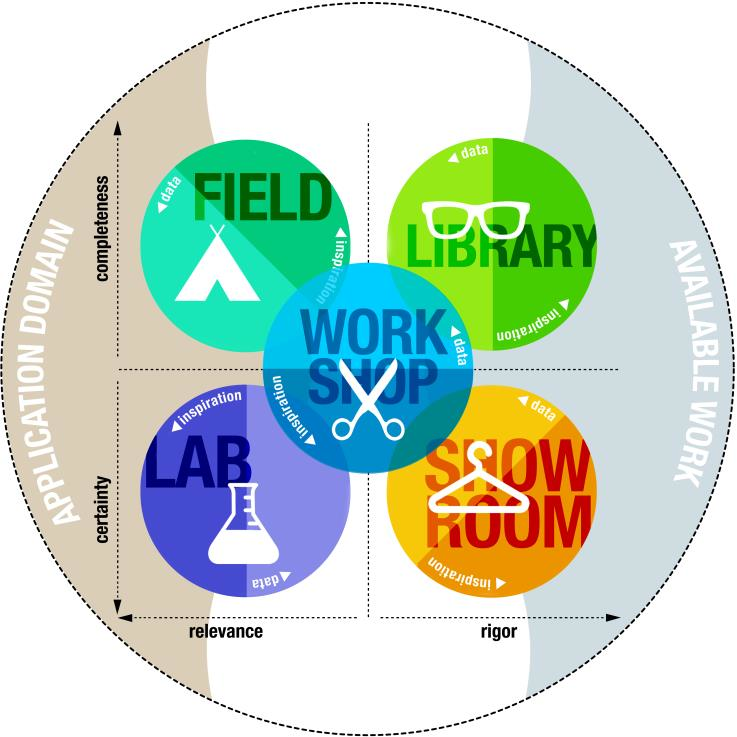
\includegraphics[width=0.48\textwidth]{figures/DOT-framework.png}
    \caption{Graphical representation of the \acrfull{dot} framework (source: \url{http://ictresearchmethods.nl/The_DOT_Framework})}
    \label{fig:dot_framework}
\end{figure}
\begin{figure}[h]
    \centering
    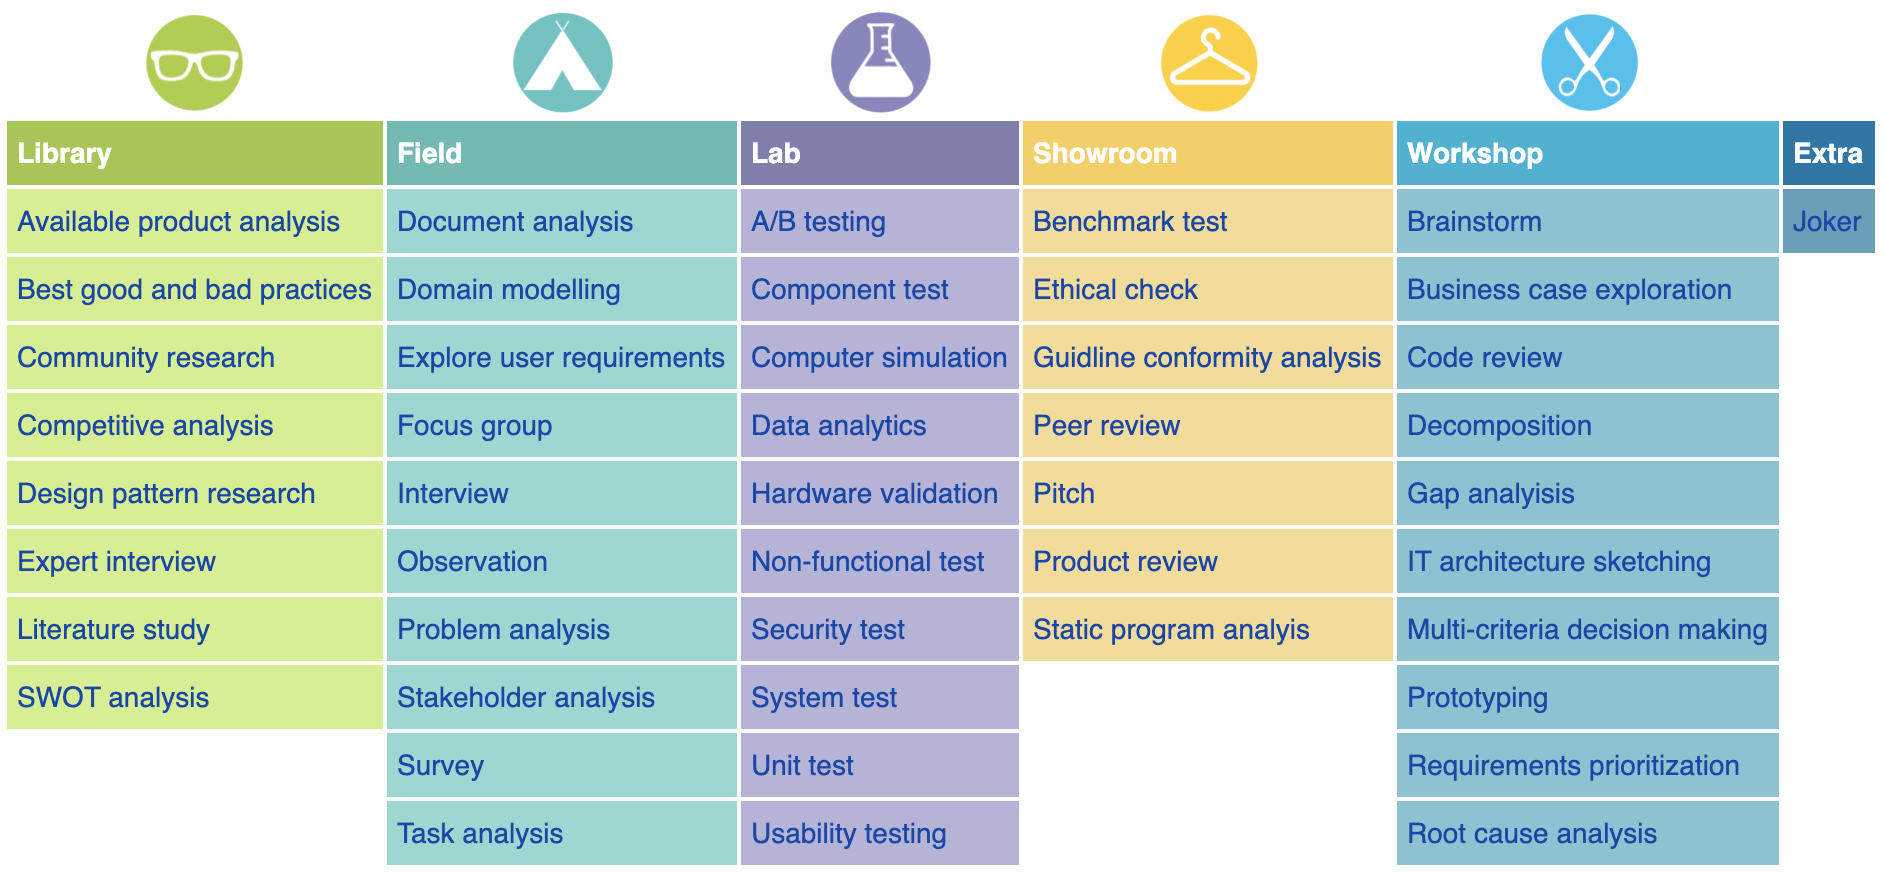
\includegraphics[width=\textwidth]{figures/dot_methods.png}
    \caption{\acrshort{dot} framework methods (source: \url{http://ictresearchmethods.nl/Methods})}
    \label{fig:dot_methods}
\end{figure}

\noindent Students are required to apply the \acrshort{dot} framework throughout their study at \acrshort{fhict}, especially when doing the internship and graduation. The following section describes the supervision of research during internship.

\subsection{Role as internship supervisor}\label{chapter:research_supervisior}
Yearly, I supervise internship students in various assignments, ranging from a more research nature to plain engineering. At \acrshort{fhict} internships are mainly external, where students can gain further experience by performing in a real work setting.
As internships are external, communication with the intern is essential to bridge client requirements and provide appropriate guidance.
Thus, the role as a internship supervisor is essentially to guide the interns in the process of understanding requirements, employing research strategies and reporting the process. 
\\\\
In this section, the supervision of an internship student previously unknown to me from the 2020 Fall semester is presented. 
I quickly derived from the first meeting that the student was proficient technically but lacked soft skills; however, was highly motivated. 
As the internship assignment was research heavy, the student expressed his concern about the planning. 
The assignment implied mainly researching  and creating a 3D head reconstruction  software, that uses pictures  of a  user  to output a 3D model for the \acrshort{vr} environment avatars. 
This feature would provide a realistic interacting between \acrshort{vr} users, preferred in the \acrshort{vr} entertainment and training endorsed by businesses.\\\\  
It is worth mentioning that throughout the internship I had a very good communication with the student via \Gls{mteams}, with report updates every two weeks.

\subsubsection{Understanding requirements}

Following the first meeting with the student where the  internship assignment was generally introduced, the first draft of the project plan was the next piece of information which helped me understand the assignment further. 
A project plan is a kind of contract between the client and the student. 
While the student needs to work autonomously during the internship project, the company guides the student in this process and needs to approve the project plan. 
The intern also discusses the project plan with the university supervisor.
This document is typically written in the first few weeks of the internship period, where the intern learns more about the company and about the assignment. 
Apart from the assignment context, the project plan includes phasing, risk analysis and a communication plan.
As an internship supervisor, I am mainly involved with the structure of the project plan and the way in which the assignment is phased. 
Also, whether the assignment objectives will be achieved is especially one of the aspects a university supervisor is concerned with.\\\\
The intern doubted whether all the assignment objectives will be achieved. 
Initially, the assignment comprised two main deliverables: a server-hosted application which can use photos of person to create and store a 3D reconstructed head model and a a mobile application that can accommodate the photo management for the server-hosted application. 
However, the project goal was mainly to create a realistic player recognition method that reconstructs the head of a person from a picture in 3D. 
Furthermore, reconstructing a 3D model from a picture required extensive research, making it already a complex task alone.
Also, the assignment context was vaguely described. While the project plan was still a fist draft, the intern had to further clarify the assignment context with the company.\\\\
As a supervisor, I had to ensure that the intern can construct a project plan accordingly. 
My main concern was the deliverables workload which could have easily resulted into two potential stand-alone internship assignments. 
As the task of 3D model reconstructing from a 2D image had a true research nature, I suggested to the intern to prioritize this in the assignment instead, since it matched the project goal. 
While the intern seemed highly motivated, a narrow assignment would better indicate realistic achievements of the internship. 
Furthermore, the intern already had optional deliverables planned for when the main task was accomplished. 
The intern confirmed shortly, after discussing assignment objectives with the company, that the focus is indeed on 3D model reconstruction, as there are no commercially available solution to perform this task and further research is required, potentially leaving less time for the other initially planned tasks.\\\\
Another concern was the formulation of the assignment context, namely current situation and assignment  problem. 
While I have an overall understanding of the technologies the intern was presenting in these segments, the project plan as well as the process report are deliverable that should be comprehensive to inexperts. 
Thus, detailed explanation of specific technologies is compulsory for a \acrshort{fhict} internship deliverable.\\\\
Sections of the the initial and final version of the project plan are shown in~\cref{appendices:research_supervising}. 
The initial version improved significantly and narrowed the intern task. This resulted into a new phasing which the intern took care accordingly. 

\subsubsection{Employing research strategies}

Regardless of the internship task, research is inevitable, and unlike academia, within \acrshort{fhict} the research is applied. 
Given the nature of the intern's assignment, the initial phase of the internship was shifted towards the research. 
The first version of the process report gave me the first insight into the intern's research approach. 
The progress report is the document interns write for the university and are assessed upon.
As the name suggests, the focus of this report will be on the process, namely how interns have come to a certain result, therefore, demonstrating that they are accountable for their actions during the assignment, and that they are able to underpin their decisions. 
Furthermore, the writing should be according to the university standard.
As a supervisor, it is my responsibility to ensure intern students have a good understanding of the research methods and their purpose. \\\\
While the intern has followed the university standards for the most part, including the \acrshort{dot} framework for applied research, the research approach was not clearly stated. 
Firstly, the research questions were missing the student presenting directly the solution. 
Each subsection of the research phase documentation could clearly be comprised into a research question, which made me comprehend that the intern had a sense of the research task but did not state the question. 
Research questions are essential to the research process. 
By defining exactly what the researcher is trying to find out,  these questions do not only dictate the trajectory of the rest of the steps taken to conduct the research but they also help anyone who may be interested in the topic to better grasp the research content. 
While they do not necessarily define where the research will end up they provide focus where the research first started.\\\\
Furthermore, the application of the \acrshort{dot} framework was incorrect, the intern stating his approach at the end of each documentation of the research task (e.i. field and lab), after specific research methods were already mentioned (e.i. interview and testing).
Stating the research approach follows right after the research questions. 
Research approaches are the plans and the procedures for research, strategies and specific methods. 
More importantly, this section is intended to show that the researcher has thought carefully about the link between the research questions and selected research methods.\\\\
In my opinion, how well a student has formulated the research approach section illustrates that the student has carefully designed and produced a sound research. 
Thus, my task was to guide the intern in formulating the main research question and sub-question and state the corresponding approach. 
I instructed the student how to formulate the research approach section, with excerpts of the feedback shown in~\cref{appendices:research_supervising}.
\\\\
It is always challenging for the interns to properly apply the \acrshort{dot} framework and document the approach. 
I have struggled myself with the framework as an \acrshort{fhict} alumna since before there was little to no instruction before the execution of the internship. 
Recently, with the introduction of personal orientation and personal development courses as well as professional skills courses in the first semesters \cite{FHICTNewCurriculum}), the knowledge of the \acrshort{dot} framework has become available much earlier. However, as a teacher of these courses, I realized students even then do not devote much effort to soft skills, being mainly interested in the technical courses.
Furthermore, there is a research based course before the graduation semester, which focuses on the application of the framework. However, this framework is also required in the internship which comes much earlier in the study. Ever since I started working within \acrshort{fhict} I highlighted the importance of applied research to all semester students and I hope that with the new curriculum, students will better carry this aspect of the education throughout their study. 
\subsubsection{Reporting the process}
At \acrshort{fhict}, during internship semesters, the students are required to write a portfolio or process report. 
In this case, the intern chose to document his process in a report format as this type of document felt more comfortable.
Essentially, a report is a short, sharp, concise document which is written for a particular purpose and audience.
Any report - whether it is about a or describing the processes of conducting research in a company - is meant for a particular type of audience. 
The audience for the internship process report is mainly \acrshort{fhict}. 
Thus, the writing has to comply to the structure and standards required by the institute. 
This involves the writing style, what to include, the language to use and the length of the document. 
Furthermore, the purpose of this report is to demonstrate the process, from understanding the problem and research questions to achieving desired results and reflecting on them.
\\\\
The intern sent regular progress updates of his document, easing the task of tracking of the process. 
Given the nature of the interns assignment, the documented progress would imply new short-term outcomes which would determine the next steps in the process.\\\\
My role as a supervisor was to provide formative feedback on each report version. More specifically I guided the intern on the following aspects of the report writing: audience, purpose, strategy, organization, style and flow. Excerpts of of the feedback are shown in~\cref{appendices:research_supervising}.
\\\\
Audience, purpose, and strategy are typically interconnected. 
When the audience knows less than the writer, the writer’s purpose is often instructional/informative. 
When the audience knows more than the writer, the writer’s purpose is usually to display familiarity, expertise, and intelligence. 
Commonly, an intern student writes a combination of both situations. 
The students need to show expertise in applying research, but may also instruct expert knowledge related to the work to help the reader fully grasp the content.
Initially, the intern composed an introductory paragraph that was well structured, however, required expert knowledge. While I am myself familiar with some of the utilized technical terms, the overall audience of a \acrshort{fhict} process report is an \acrshort{ict} professional that is fairly informed about existing technology but not necessarily expert. Therefore, specific terms and technologies require further explanation to fully understand the content.
\\\\
Readers have the expectation that information will be presented in a structured
format that is appropriate for the particular type of text. At \acrshort{fhict} the internship report should be organized in specific chapter and sections, such as \textit{Introduction}, \textit{About company} and \textit{Process}. While the intern presented the progress results in sections of the \textit{Process} chapter, the main outcome of the internship was difficult to locate. Therefore, a final \textit{Result} chapter that summarizes the main outcomes is necessary, especially to prove whether the research question and sub-questions were answered. The intern managed to formulate this chapter after several feedback meetings.
\\\\
Furthermore, students need to be sure that their communications are written in the appropriate style. 
A formal report written in informal English may be considered simplistic, even if the actual ideas and/or data are complex.
Moreover, students have to be aware of the stylistic advice within the institute.
The intern had an expected stylistic communication in the report.
For example, some processes and procedures were not described with passive voice. 
Although aware, sometimes the intern used contractions (short forms) \textit{don't}, \textit{aren't}, \textit{shouldn't}.
In the case of the \textit{I} pronoun, the intern appeared to overuse it, while this is usually present in an \acrshort{ict} related report to support and emphasise own point or outcome. I highlighted these stylistic suggestions once and let the intern decide whether or not they will be modified/used in the rest of the writing.
\\\\
Another important consideration for successful communication is flow,
moving from one statement to another. Naturally, establishing a
clear connection of ideas is important to help the reader follow the text. Linking words, such as \textit{furthermore}, \textit{moreover}, \textit{however} usually provide this flow. The intern lacked in linking words and had some misuse of punctuation, which were specified in the feedback.
\\\\
With every internship I take an instructional position in the report writing process. I especially take this instructional position during the first internship to help students better prepare for the graduation internship report. This intern was always eager to receive and incorporate feedback. While the intern was already at a satisfactory level, I provided feedback on every writing aspect that could be improved and let the intern decide whether to use my recommendations or not. I am content with the intern's progress in terms of writing which will be essential not only in the following internship, but also after graduation.









% \section{Research assessment}\label{chapter:research_assessment}
% \subsection{Role as internship assessor}\label{subsection:role_internship_assessor}
At \acrshort{fhict}, the internship/graduation internship assessment is paired, summing the opinion of the supervisor and a second assessor evaluating only the final version of the internship report. Assessors align their evaluation on the intern's report and a general agreed assessment is formed. Then, the assessment is further discussed and aligned with the other parties, such as company supervisor and external assessor (only in graduation), at the time of the internship assessment (e.i. final presentation meeting).
\\\\
As a supervisor, a general assessment is usually formed from the first few feedback sessions. The intern I discuss in~\cref{chapter:research_supervisior} had a satisfactory report which with feedback proved great improvement in the final version. This is usually how the students perform in the writing part of the internship. I always pride myself with students that understand the importance of the written assessment and succeed to improve and deliver better documentation. After discussing the report with the second assessor, the writing was assessed to 8.5 out of 10, the student scoring overall a higher than average grade (considering work and presentation/defense), namely of 9 out of 10.
\\\\
Apart from assessing interns I supervised, I also took the role of second assessor in both internships and graduation internships.
While the second assessor role was introduced later in the internship assessment as it already existed in the latter, I believe that it is very favorable to assess reports other than the own supervised intern reports.
On the first semester of the academic year 2019-2020 I took this role for several students. My opinions on these reports is shown in~\cref{appendices:internship_report_appendix}. One student had a poor final process report, although the delivered work was sufficient. 
The internship assignment involved developing a prototype to fully automate a heavily manual operated application to then to test for viability against the original. 
After consulting the supervisor, the student was given a second chance to fix the report grade, scoring initially a 5 out of 10, which is a fail. 
First, the student delivered a journal like report, with weekly updates and implementation details which could have been better written in the appendix. 
Overall, the report read difficult and did not satisfy the \acrshort{fhict} standards. 
For instance, the research approach and research questions were not clearly stated. 
Also, the information about research and development was disrupted into two main sections instead of one process, proving that the student was unaware of how to apply the \acrshort{dot} framework. 
With the second attempt the student managed to incorporate some of the feedback and pass with a 5.5 out of 10. 
\\\\
Another student was assessed poorly due to the overall report structure, although the content was generally understandable.
The internship assignment concerned implementing different tasks to an already existing application, including bug fixes, new feature implementations, testing and experimenting with new tools and technologies.
While this time, this student had stated a research strategy, the research questions were missing. 
Furthermore, the report was structured as a journal and included implementation details which do not add the the overall understanding of the process. 
After consulting the supervisor, the student was assessed with 6 out of 10 for the report.
\\\\
At the end of the academic year 2019-2020 I was the second assessor of two graduation interns. My opinions on these reports is shown in~\cref{appendices:research_assessing_graduation}.
The first graduate intern was assessed in June 2020. 
The graduate developed a new format for survey specifications that reduces the complexity of code syntax, using spoken language instead. 
While the assignment was carried out during the COVID-19 outbreak, the graduate managed to achieve the main objectives in rather special circumstances (e.i. home work and little to none company interaction).
Since this was the first time I handled a graduation report, I initially observed my co-assessor's opinions about the writing.
I quickly learned that generally we shared the same opinions. 
While the writing was understandable, the main issue was that the graduate included details that should not be part of a process report, but better for a user manual. 
For example, the intern had snippets of code in a specific programming language, where usually algorithmic statements are presented in a process report in pseudo-code at most. 
Furthermore, the reading was complex and heavy in technical terms, which could have been eased with inclusion of more graphical representation of the processes. 
I was surprised to discover that the supervisor did not see a complete final draft of the report before. 
Given the immense improvement compared to the previous report version noted by to the graduate supervisor, the report was graded with 7 out of 10, which indicates generally an average performance (e.i. as expected).
\\\\
In August 2020 the second graduate intern was assessed. While the graduations take place before July in the second semester of the academic year, this intern had a delay due to health issues. The graduate conducted extensive research to develop a fully digitized medical whiteboard.
The report described the activities and the way of working sufficiently, however, more technical details would have been expected in the appendix. 
Furthermore, some issues, such as contractions, typos and grammar mistakes could have been easily avoided if the student would have double checked the text. After discussing with the supervisor, the report was assessed with 7 out of 10.
\subsection{Role as project assessor} \label{subsection:role_project_assessor}
The second semester students from ICT \& Software Engineering are introduced to research and the \acrshort{dot} framework during the execution of a group project. 
The project is a software management solution for a shop that keeps track of employees and products, on the basis of proper software design. 
The students research an optimal software architecture to accomplish the project requirements. 
Furthermore, the students work for a client under the supervision of a tutor, roles fulfilled by two different teachers. 
While the supervisor is observing the process and guiding groups through roadblocks when required, the client is not be aware of any of the technical aspects and meets the groups few times to specify project requirements.
I took the role of both client and supervisor for the academic year 2019-2020 second semester, which was the first iteration in the new curriculum. While I supervised three groups and acted as the client for other three groups, below I discuss groups from each role.
\\\\
As a project supervisor, I assess groups on their process, documentation and deliverables, verifying also the technical side of the delivered products. One of my groups had communication issues between the members, with two students performing outstanding and the other two slacking constantly. It is also worth mentioning that the students are sufferers of the COVID-19 outbreak online education, which has affected their group work routine. Initially the work and deliverables were poorer, however, based on feedback, the students improved. I focused especially on the architecture design (e.i. \acrshort{uml} diagram), being the core knowledge the students acquire in the ICT \& Software Engineering second semester. The group especially improved their soft skills, namely presentation and report writing, as I emphasised the importance of these skills for the \acrshort{fhict} assessment but also after the graduation. While the formative indications as a group progressed from S(Satisfactory) to O(Outstanding)\footnote{In the new curriculum letter grading is used instead: P(Poor), U(Unsatisfactory), S(Satisfactory), G(Good), O(Outstanding)}, the group even impressing the client with extra features, the slacking students were assessed lower, to just a S. An excerpt of this group's process report is shown in~\cref{appendices:research_assessing_project}.
\\\\
As a client, I assess the groups on how they conduct meetings, if they ask the right questions and if they deliver what they promised. 
Unlike the supervisor, I will assess products on a shallow level (e.i. only at the user experience). One of the groups that impressed me from the beginning with researched solutions and prototypes exceeded in my opinion the second semester learning goals. While I could see room for improvement in the documentation, this group was assessed O throughout all the three formative indication moments, satisfying all the requirements that were asked from me as a client. In contrast, another group underdelivered throughout the project, despite the continuous feedback and support. Initially formed out of four students, the group dissolved during the project execution, leaving only one member active. This was a challenging group to assess, however, together with the project tutor it was decided to lower the project requirements and give the student a chance to achieve at least a S, and, thus, pass the project. While the majority of the work was already done by the one student which was left in the group, the student was suggested to focus on testing already existing features and deliver a robust solution with less functionality than initially promised. 
\\\\
It is challenging for me to act as a client in these projects as I am always driven to tutor students when they can improve. For the poor group for which I acted as a client, it was difficult for me not give tutor feedback, however, at each formative indication moment I discussed improvements with the tutor and shared our feedback collectively. Examples from my assessment feedback for these groups is shown in~\cref{appendices:research_assessing_project}.

\section{International Students Writing Skills: An Investigation}\label{chapter:research_expertise}
\subsubsection{Introduction}\label{chapter:research_introduction}
In any higher professional education context, the student population is expected to adopt an academic discourse to satisfy the requirements of successful communication. 
The discourse usually takes the form of presentations, feedback or writing. 
\\\\
Writing tasks constitute a major component in any higher professional education setting.
At \acrshort{fhict}, an undergraduate is expected to demonstrate writing skills as part of their professional skills defined by the HBO-i framework through a large variety of written tasks.  
These tasks become progressively complex, from writing project documentation (i.e. a project plan or user requirements specification in early internal projects), to writing process reports that describe the applied research methodology (i.e. process report/portfolio during internship and graduation with partners in education).
However, many students are either unaware of the importance of writing in academic discourse or do not know what exactly constitutes academic writing.
Studies such as \citeauthor{Lillis2001} and \citeauthor{Elander2006} have argued that students may fail to demonstrate satisfactory writing skills due to the university not explaining and teaching its discourse practices and conventions explicitly enough.
\\\\
This study aims to raise awareness amongst the \acrshort{fhict} teachers and offer suggestions as to better facilitate the students’ development of writing skills.
In order to establish a background and a frame of reference for the study, a review of a range of academic writing considerations is presented. 
After discussing the methodological approaches which underline the study, the findings are discussed.
Finally, the conclusion brings together the most relevant insights which emerged from the research and outline some implications for the current academic context. 

% \subsubsection{Problem definition}\label{chapter:research_hypothesis}
%  

% or the last five iterations of the course I have been experimenting with several course material types. 
% From slides to additional lecture notes, each iteration had some implementation of the student feedback. 
Thus, the hypothesis was defined as follows:
\textit{Students who receive proper training in writing practices and conventions explicitly enough improve overall writing professional skills.}


\subsubsection{Academic writing}\label{chapter:research_preliminaries}
\begin{figure}[t]
    \centering
   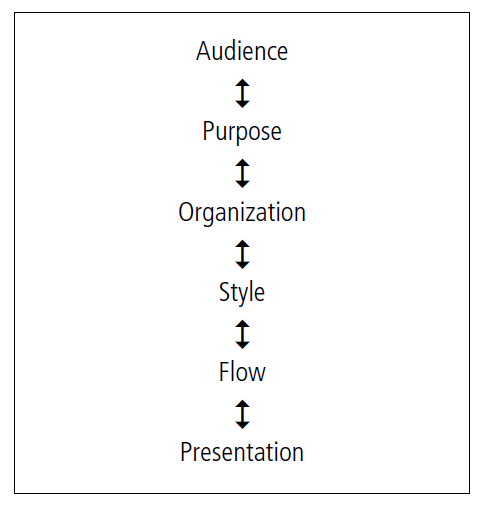
\includegraphics[width=0.5\textwidth]{figures/research/writing_considerations.PNG}
    \caption{Considerations in Academic Writing~\cite{Swales2012}}
    \label{fig:writing_considerations}
\end{figure}

According to~\citeauthor{Swales2012}, academic writing is a product of many considerations which can be categorized in five units: audience, purpose, organization, style, flow, and presentation (see Figure \ref{fig:writing_considerations}).
Audience and purpose are typically interconnected. The first consideration towards a successful writing is to identify the audience. 
For most students, the audience will be a tutor presumably knowledgeable about the writing topic. 
Other possible audiences include external experts (i.e. partners in education) and graduation committees (i.e. those who will review and assess graduation dissertations, usually university staff and external experts). 
Understanding the audience will better define a writer's purpose and strategy (or strategies). If the audience knows less than the writer, the writer’s purpose is often instructional (as in a manual). 
If the audience knows more than the writer, the writer’s purpose is usually to display familiarity, expertise, and intelligence. The latter is a common situation for the undergraduate student writer.
\\\\
Academic writing has also expected patterns of organizing the information for a particular type of text. 
A type of text is referred to as general-specific, which can be used to produce an introduction paragraph or definitions. 
As the name suggests, these texts involve moving from broader statements to more specific ones. 
The opposite of general-specific is specific-to-general texts, which can structure conclusions and recommendations. 
An important text pattern is the problem-to-solution, especially since academic research focuses on solving problems. 
A problem-to-solution structured text is usually presenting the situation, reasons the problem, discusses ways to alleviate the problem and then evaluates proposed solution(s).
However, often an incomplete solution is offered which may introduce a new problem that will then be addressed similarly. 
Other ways of organizing text enumerate comparison-contrast, cause-effect and classification~\cite{Swales2012}.
\\\\
One difficulty of undergraduate student writers in using the appropriate style. 
Most aiding tools and programs are written primarily to find spelling and basic grammar errors, not to offer stylistic advice for academic writing.
While  stylistic conventions differ in every field, most common stylistic conventions in the field of \acrshort{ict} enumerate: passive voice, addressing the reader (i.e. You can see the results in Table 1), contractions (i.e. don't, isn't), language that softens a point (i.e. may, appears to), concise sentences (i.e. nominalization).
\\\\
Another important consideration for successful communication is flow: moving from one statement in a text to the next. Naturally, establishing a clear connection of ideas is important to help the reader follow the text. 
Although most writers' first instinct is to use logical connectors (i.e. however or furthermore), following a progression from old or given information to new information is generally preferred
Placing relevant 'old' information in early position establishes a content connection backward and provides a forward content link that establishes the context. 
Furthermore, logical connectors rise the issue of punctuation.
Many general style guides and style guides are specific to a  field of study, however, most common punctuation enumerate: semicolons (;), colons (:), dashes (—), and commas (,).
\\\\
Finally, and most importantly, the presentation of a writing task is key in academic writing.
Most instructors tolerate small errors in language in papers written by nonnative speakers—for example, mistakes in article or preposition usage. 
However, errors that instructors think could have been avoided by careful proofreading are generally considered less acceptable.
Thus, an instructor's focus should be more on content and information flow first rather then grammar or text formatting.
\\\\
\textit{Writing research}
\\\\
Research governs academic writing. 
While there are different types of research as well as different types of research writing, several text formatting aspects are expected in an academic research writing.
The content generally follows the standard Introduction-Method-Result-Discussion (IMRD) pattern. 
As shown in Figure \ref{fig:research_writing_formatting}, the arrows indicate that the sections are closely connected, moving from generals-specific to specific-to-general information.
The main purpose of the Introduction is to provide the rationale for the research, moving from a general discussion of the topic to the particular question, issue, or hypothesis being investigated. but also to attract interest in the topic-and hence readers.
The Methods section describes, in various degrees of detail, methodology and materials, while in the Results section, the findings are described, accompanied by variable amounts of commentary.
The Discussion section gives meaning to and interprets the results in a variety of ways, referring to statements made in the Introduction.
Furthermore, most frequent writing considerations encountered in IMRD are shown in Table \ref{table:frequent_writing_considerations}.

\begin{figure}[t]
    \centering
   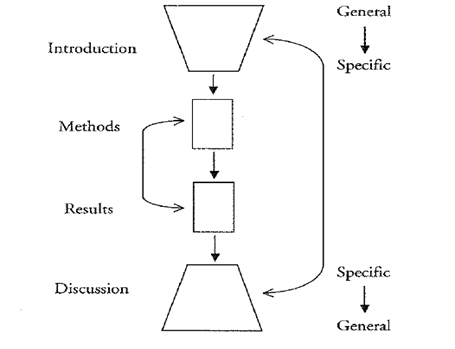
\includegraphics[width=0.65\textwidth]{figures/research/research_writing_formatting.png}
    \caption{Overall Research Writing Structure~\cite{Swales2012}}
    \label{fig:research_writing_formatting}
\end{figure}

\begin{table*}[t]
\centering
\caption{Frequent Academic Writing Considerations}
\begin{tabular}{|l|l|l|l|l|}
 \hline
     & \textbf{Introduction} & \textbf{Methods} & \textbf{Results} & \textbf{Discussion} \\
 \hline
    Present tense & high & low & low & high \\
 \hline 
    Past tense & mid & high & high & mid \\
 \hline
    Present perfect & mid & low & low & mid \\
 \hline 
    Passive & low & high & variable & variable \\
 \hline
    Citations & mid & mid & variable & mid \\
 \hline
    Hedging & mid & low & mid & high \\
 \hline
\end{tabular}
\label{table:frequent_writing_considerations}
\end{table*}


\subsubsection{Methods}\label{chapter:research_method}
% \subsubsection{Data collection}\label{chapter:research_method_data_collection}

% An \acrshort{ale} student group that received both versions of the course with and without instructional materials was utilized.

%2020: 168 +  2019: 82 + 2018: 43 = 293
The investigation was carried out with \acrshort{fhict} teachers and undergraduate students. 
To identify teacher' experience with assessing writing tasks, 41 teachers with at least one year of experience within the \acrshort{fhict} education were given an Writing Skills Assessment  Questionnaire (appendix~\ref{appendix:writing_skills_assessment_questionnaire}).
To identify students’ perception and understanding of writing, three cohorts (2018, 2019, and 2020) with a total of 293 undergraduates were given a Writing Skills Questionnaire (appendix~~\ref{appendix:writing_skills_questionnaire}). 
These cohorts comprised students in their third-year and forth-year of studies enrolled in either internship, electives and graduation. 
In addition to close-response items to elicit information on students’ background and experience, there were several open-ended questions to acquire in-depth information on experiences of both assessors and students.
Some open-ended question asked directly ‘Can you state other writing consideration you know than those mentioned above? Try to state as many as possible.’ or 'Do you think students require further attention in improving writing skills? If yes, can you state what should be improved.'.
\\\\
Students' writing skills were investigated through the analyses of internship and graduation assessments. The analysis included 57 alumni (cohort 2017) were scores for assignment execution, writing, and presentation and defence were considered from both internship and graduation assignments. The analysis focused on identifying significant progress in students' writing based on prior experience from internship to graduation.
\\\\
As part of a wider investigation,
48 internship reports of third-year students (cohort 2019) were analysed. The analysis focused on the writing guidelines students referred in the development of their writing task. These guidelines include report writing guidelines handbook for internship and graduation  as well topics presented during the old curriculum course \acrfull{popd}~\cite{fhictpopd2} (applies to students who have started a study program at \acrshort{fhict} up to and including the spring of 2019).


\subsubsection{Findings and discussion}\label{chapter:research_results}
\textit{Student's concept of writing}\label{chapter:research_results_students_findings}
\input{chapters/research/research_expertise/research_results/research_results_students_findings}
\textit{Teacher's concept of writing}
\label{chapter:research_results_teacher_findings}
\input{chapters/research/research_expertise/research_results/research_results_teacher_findings}
\textit{Limitations in teaching academic writing}
\label{chapter:research_results_limitations}
\input{chapters/research/research_expertise/research_results/research_results_limitations}
\textit{Improving teaching academic writing}
\label{chapter:research_results_improvements}
\input{chapters/research/research_expertise/research_results/research_results_improvements}


% \begin{table*}[t]
% \centering
% \caption{Pre-development and post-development of the \acrshort{ale} course material per student group with results of statistical analyses}
% \resizebox{\textwidth}{!}{%
% \begin{tabular}{p{3.5cm} p{3.5cm} p{3.5cm} p{3.5cm}}
%  \hline
%      & Cumulative ALE score 
%      %Mean $\%$ score ($\pm$ SD)
%      $N$ &  ANOVA test comparing group performance & Kruskal Wallis H test  comparing group performance \\
%     \hline
%     Control group  & 50 & $p>0.1$ & $p>0.1$ \\
%     (pre-development)&&&\\
%     Test group     &1 & - & -  \\ 
%     (post-development)&&&\\
% \hline
% $N$ number of students&&&\\
% \end{tabular}%
% }
% \label{table:statistical_analysis_scores_different_groups}
% \end{table*}

% \Cref{table:statistical_analysis_scores_different_groups}  and \Cref{table:statistical_analysis_scores_same_group} show the results of the statistical analyses tests performed in this study.
% First, a comparison between past \acrshort{ale} iteration was made to identify differences.
% \Cref{fig:distribution1820} shows the score distribution for pre-development course material student groups. 
% To satisfy the ANOVA independency condition, students which attended both \acrshort{ale}1 and \acrshort{ale}2 had their scores averaged, yielding to each group containing independent samples. 
% While data is normal, group 1920ss is positively skewed. 
% Assuming normality, with ANOVA the $p$-value is greater than 0.1. With Kruskal Wallis H-test the $p$-value also exceeds 0.1, thus, in conclusion, there is no statistical difference between the scores of previous \acrshort{ale} course iterations. The post-development group was also included and tested with ANOVA and Kruskal Wallis H. Similarly, student scores from group 22021fw were averaged to satisfy independency.\\\\
% %However, no significant difference was identified with the post-development comparison.\\\\
% %The paired t-test was conducted on the 22021fw which had both pre-development and post-development course material.[TODO]\\\\
% %\Cref{fig:distribution2021fw} shows the score distribution for the pre and post-development course material. [TODO]\\\\
% %This test yielded a $p<0.05$ which indicates that there is a significant difference between student performance with the new course material.
% %Looking at the distribution it is clear that 2021fw2 group performed better. \\\\
% Furthermore, there is not significant difference in the performance of past \acrshort{ale} student groups.
% \Cref{appendices:scores} describes a detailed study of the test group 1920ss for which the statistical analysis proved significant evidence in comparing \acrshort{ale}1 with \acrshort{ale}2 performance. For this group, although there seems to be a difference in performance, the performance in \acrshort{ale}2 is worse due to the introduction of weekly deadlines and mandatory feedback sessions. Moreover, having participated in the \acrshort{ale}1 course, the students should be familiar with the workload and requirements. However, while a few students score slightly better, majority seems to perform worse in \acrshort{ale}2. This may also be due to the fact that students usually join some electives to fill in missing \Gls{ec}s and deliver up to a passing grade. Thus, further research is required to assess student performance in both \acrshort{ALE} courses. Also, the study should be performed on larger groups, as the current test group was too formed of too little students.\\\\
% Unfortunately, the second part of the course had one student left for assessment. While several students joined in the beginning, majority dropped till the end, yielding a test group formed of 1 student that has followed both \acrshort{ale}1 and \acrshort{ale}2. Hence, the statistical testing could not be performed anymore for this test group.


% \begin{table*}[t]
% \centering
% \caption{\acrshort{ale} scores per student group with results of statistical analyses}
% \resizebox{\textwidth}{!}{%
% \begin{tabular}{p{3.5cm} p{3.5cm} p{3.5cm} p{3.5cm}}
%  \hline
%      & Cumulative ALE score Mean $\%$ score ($\pm$ SD) $N$ &  Paired t-test comparing ALE1 with ALE2 performance &  Wilcoxon signed-rank test comparing ALE1 with ALE2 performance\\
%  \hline
%     1718ss & $7.97\pm1.26$ & $p>0.1$ &\\
%     &5&&\\
%     1819fw & $8.78\pm0.78$& &  $p>0.1$\\
%     &8&&\\
%     1819ss & $8.33\pm0.69$& $p>0.1$ &\\
%     &8&&\\
%     1920fw & $8.25\pm1.25$& - &  -\\
%     &1&&\\
%     1920ss & $7.3\pm1.22$& & $p<0.05$\\
%     &10&&\\
%     2021fw & & -& -\\
%     &1&&\\
%      \hline
% SD standard deviation, & $N$ number of students&&\\
% \end{tabular}%
% }
% \label{table:statistical_analysis_scores_same_group}
% \end{table*}


% \begin{figure}[h]
%     \centering
%     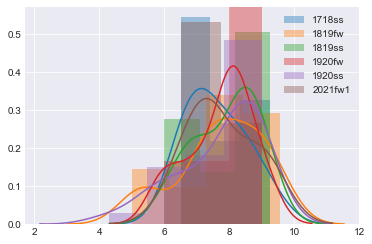
\includegraphics[width=0.7\textwidth]{figures/distribution.png}
%     \caption{\acrshort{ale} integral assessment scores distribution for the 2018-2020 student groups}
%     \label{fig:distribution1820}
% \end{figure}
% % \begin{figure}[h]
% %     \centering
% %     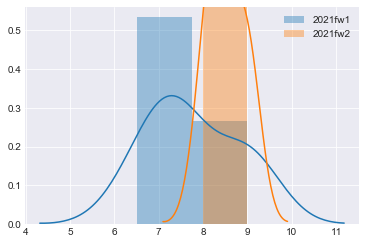
\includegraphics[width=0.7\textwidth]{figures/distribution2021fw-mock.png}
% %     \caption{\acrshort{ale} integral assessment scores distribution for the 2020-2021 Fall/Winter semester student group}
% %     \label{fig:distribution2021fw}
% % \end{figure}

\subsubsection{Conclusion}\label{chapter:research_conclusion}
This study has presented an extensive analysis over the student performance influenced by course materials in the fourth year elective \acrshort{ale}. 
While there is not enough statistical significance to confirm that the performance was positively influenced due to redevelopment of course materials, there is a slight improvement. 
Further research is required to collect further statistical evidence from future \acrshort{ale} iterations. 
Regardless, course material should be continuously tailored to the students as it it the canvas to which scholars build their learning.

% \section{Reflection}\label{chapter:research_reflection}
% In my opinion, research is an essential part of a modern \acrshort{ict} professional. 
While I knew about applied research as an alumna, I learned further about the integration of research throughout the entire four year study programme at \acrshort{fhict}. 
This has especially became obvious to me while teaching in the new curriculum in the academic year 2019-2020, since before it was less notable. 
As students advance in their study in the new curriculum, they learn progressively about applied research as a professional task. 
Thus, I believe that if consistently addressed, the research task will become easier for students in their internships and graduation internships, unlike old curriculum students, which were introduced to research later.\\\\
Furthermore, revising the \acrshort{dot} framework has made me a better supervisor. 
While I carry many aspects of reporting from the basic/fundamental research experience in my supervision, it is always good to revise the institute research framework. Lately, students have become more professional in employing the framework as a result of more research oriented courses in the new curriculum; however, I always find they lack soft skills. Especially for the first internship, students often struggle in documenting their process. I try to be as explicit and through in providing feedback, especially related to writing. Furthermore, I have learned to adapt and accept repetitive mistakes even after receiving thorough feedback. While I strive for all students to succeed in all aspects, I learned to become more accepting of students being less concerned of their writing skill and adapted my feedback accordingly. 
\\\\
Lastly, undergoing the task of portraying research expertise was one of my favourite tasks in this portfolio. The example presented shows just one of the situation where I employ my research skills in my teaching. As I plan to pursue a PhD career in the near future, personally, research is always an exciting and stimulating task.





\clearemptydoublepage

\chapter{Conclusions}\label{chapter:conclusions}
The aim of this portfolio was to prove professionalism within education at \acrshort{fhict} through didactics, testing and \acrshort{tel}, as well as research. 
As a pedagogue, didactical skills are continuously developed to adapt to the scholars and institute demands. 
Furthermore, a pedagogue should adapt education according to the industry's (e.i. enterprises or organizations) demands to train industry prepared professionals.
\\\\
The evidence presented in this portfolio is the result of the past three years of activity within the institute. Having performed several roles already (e.i. lecturer, assessor and internship tutor), the task of didactics development and research presented in this work were well received. 
As part of the didactics, testing and \acrshort{tel}, the redevelopment of course materials for a fourth year ICT \& Software Engineering elective was presented. 
This redevelopment motivation was well backed up by personal experience as well as student feedback. 
The course was fully revised using the \acrshort{soo} model, including revision of learning outcomes according to the Learning Outcomes Manual~\cite{learningoutcomesmanual}.
Furthermore, the \acrshort{fhict} assessment policy~\cite{FHICTAssesmentPolicy} was followed in the creation of the course assessment. 
The course was then physically published through \acrshort{tel} means (e.i. lecture slides, course notes and exercise files) onto \gls{canvas}, \acrshort{fhict}'s online \acrshort{lms}.
Parallelly, the research task was undertaken where research expertise as well as research supervision activity in internal and external projects was presented. The task of supervision was described through examples, as well as assessments. Furthermore, as research expertise, a study of student performance based on developed course material was presented. 
\\\\
Overall, I believe this work has improved my didactical skills and has made me a better \acrshort{fhict} pedagogue. First of all, learning about various sources of information that the institute offers about the education has been eye opening. While reading about policies and rules has helped me become more confident in my employed didactics and the quality of education, it has also paved a strong background about curriculum development and course design tasks which I am willing to shoulder. Furthermore, research will always be my passion, thus, I would continuously look for opportunities to improve personally and also improve education.

\clearemptydoublepage

%Choose a good bibliography style, plain would do often, but these might be nice too
%\bibliographystyle{these}
%\bibliographystyle{plainurl}
\bibliographystyle{unsrtnat}
\bibliography{references}

\clearemptydoublepage

\appendix
\addcontentsline{toc}{chapter}{Appendix}
\chapter{Writing skills module - Proposal}\label{appendix:proposal}
This appendix shows the writing skills module proposal shared with the responsible teaching staff from each of the five Semester 3 profiles, namely Software, Technology, Business, Media and Infrastructure.

\null\hfill (See next page)
 
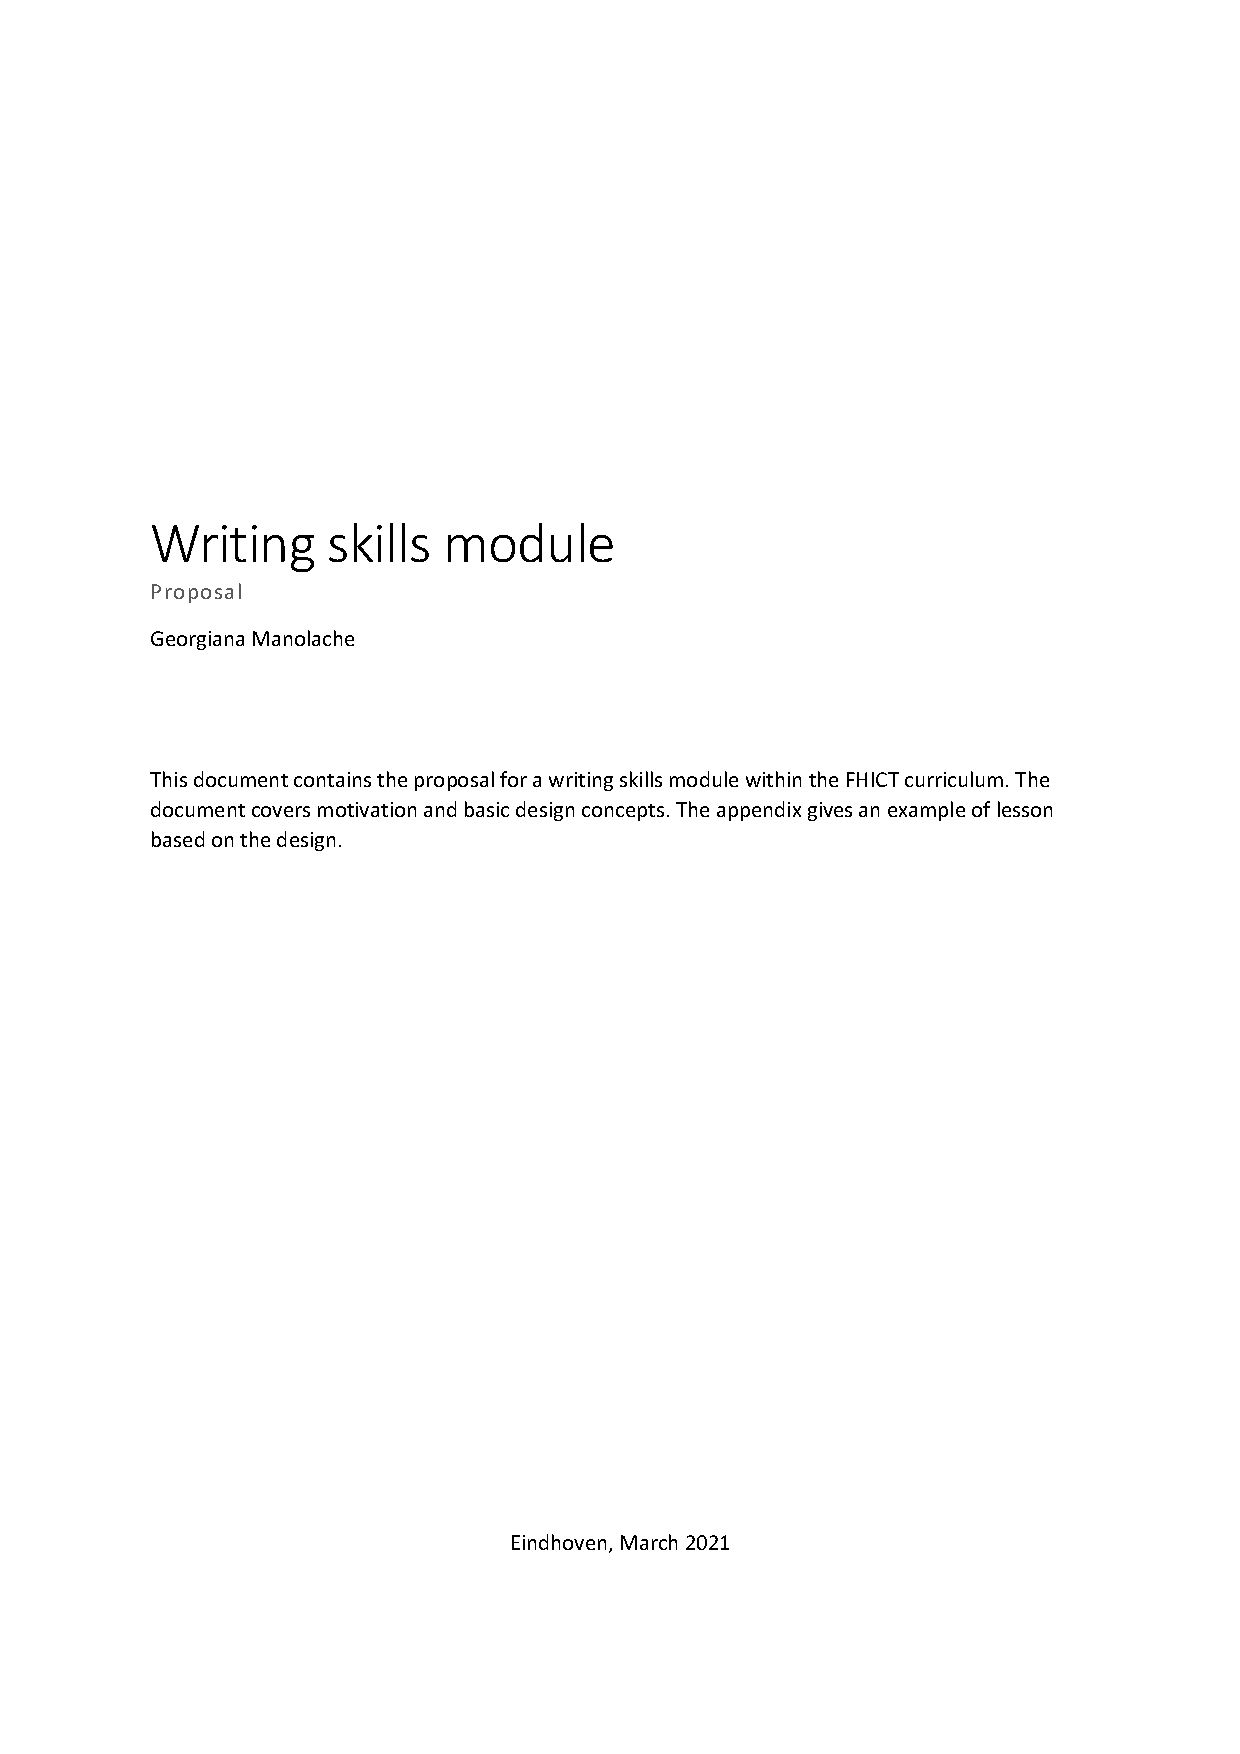
\includepdf[pages=-]{appendices/proposal/Writing_Skills_Module-Porposal.pdf}



\chapter{Writing Skills Assessment Questionnaire}\label{appendix:writing_skills_assessment_questionnaire}
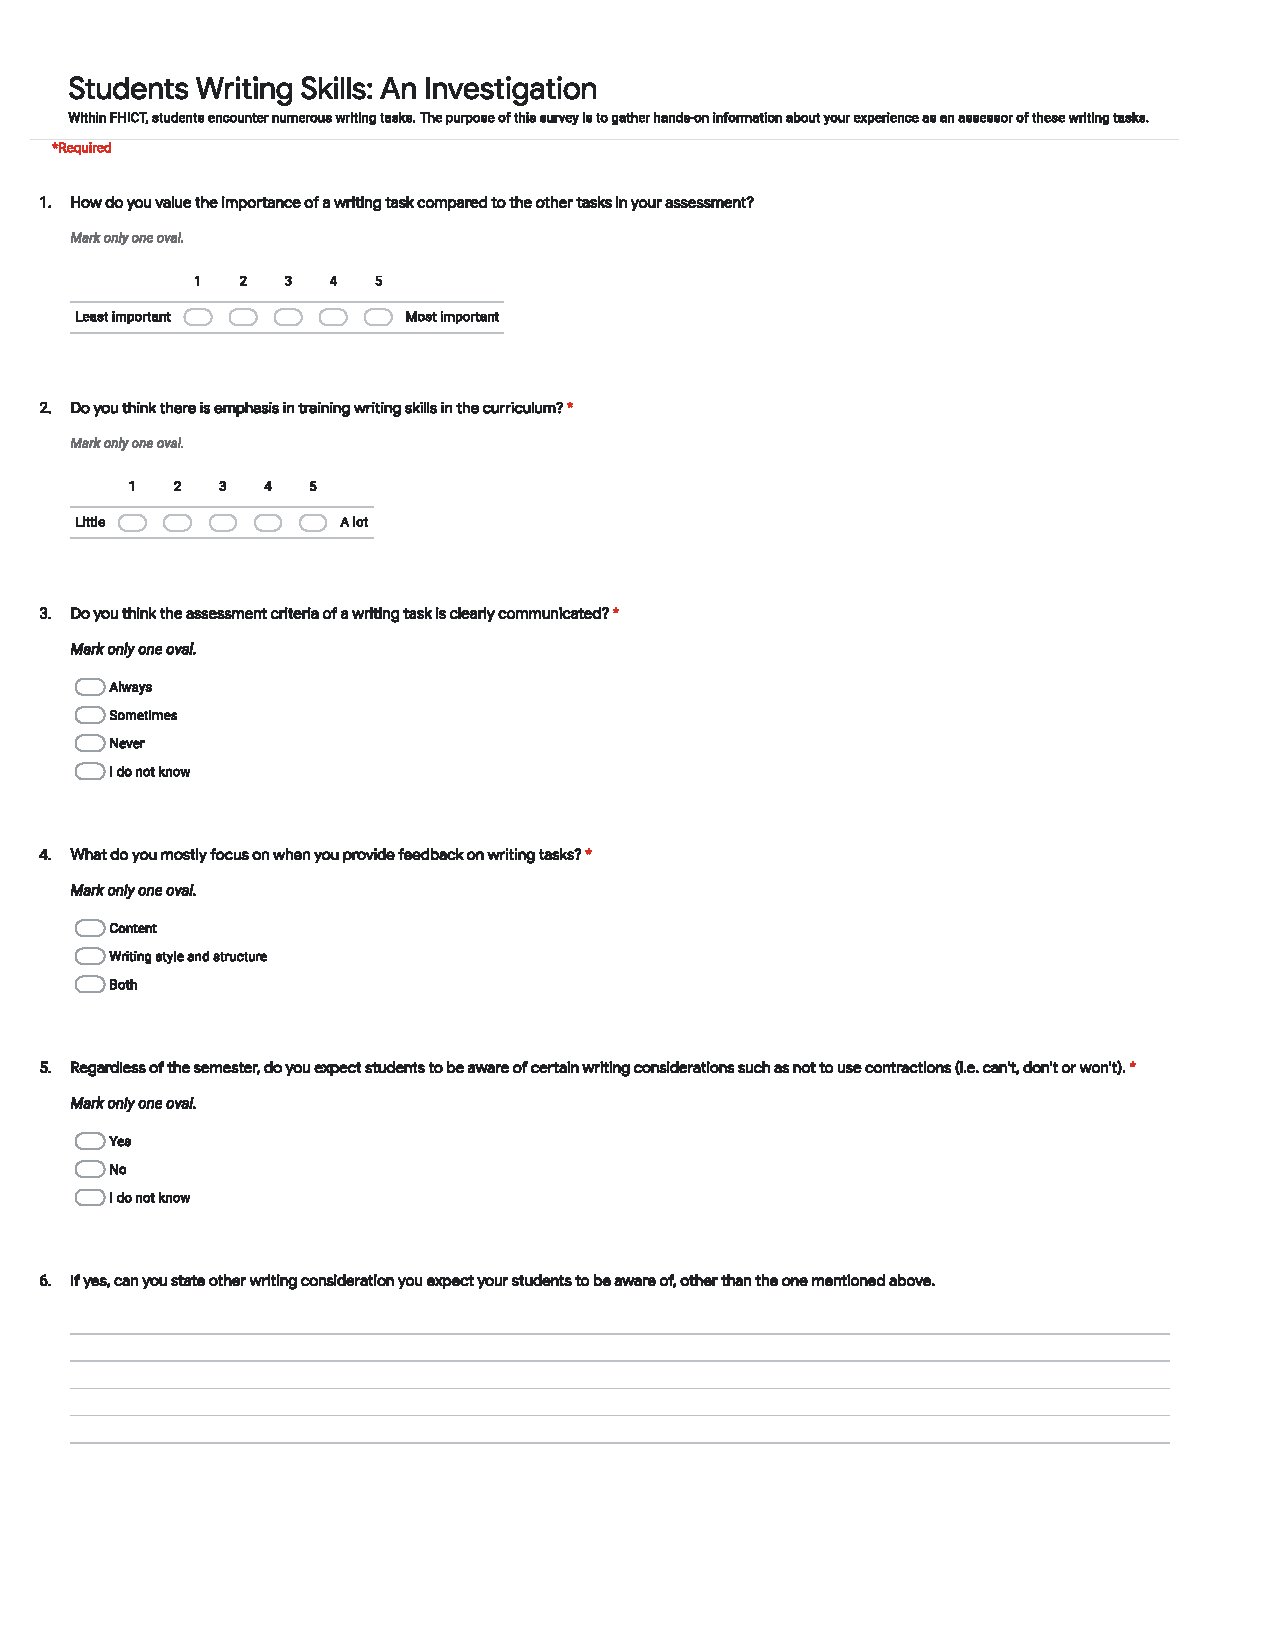
\includepdf[pages=-]{appendices/research/questionnaire/writing_skills_assessment_questionnaire.pdf}

\chapter{Writing Skills Questionnaire}\label{appendix:writing_skills_questionnaire}
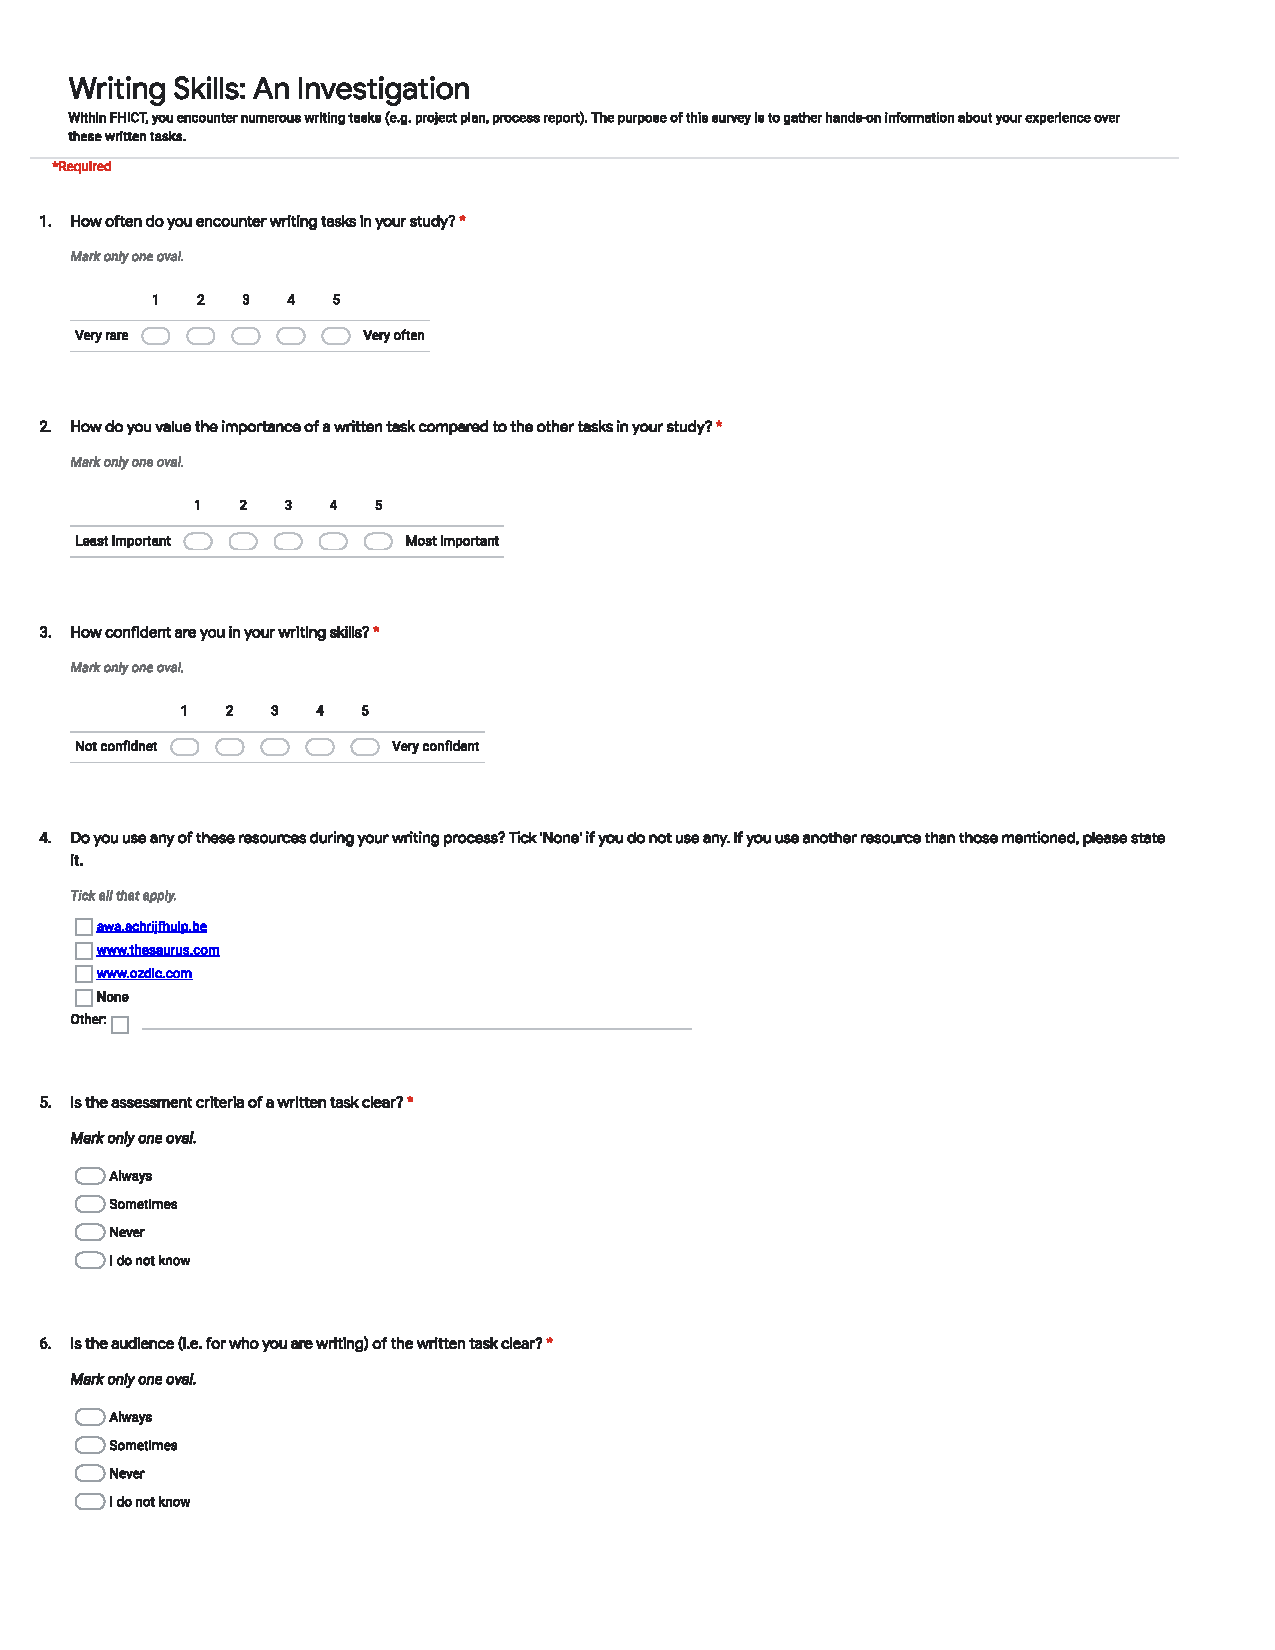
\includepdf[pages=-]{appendices/research/questionnaire/writing_skills_questionnaire.pdf}

\end{document}
